

\documentclass[JIP]{ipsj_v2/UTF8/ipsj}

\usepackage[dvipdfmx]{graphicx}
\usepackage{latexsym}
\usepackage{amssymb}
\usepackage{float}
\usepackage{enumerate,cite,url}
\usepackage{color}
\usepackage{listings,jlisting}
\lstset{%
    language={c},%
    basicstyle={\footnotesize\ttfamily},%
    identifierstyle={\footnotesize},%
    commentstyle={\scriptsize\itshape},%
    keywordstyle={\footnotesize},%\bfseries},%
    ndkeywordstyle={\footnotesize},%
    stringstyle={\footnotesize\it},
    frame={tb},
    breaklines=true,
    columns=[l]{fullflexible},%
    numbers=left,%
    xrightmargin=0zw,%
    xleftmargin=3zw,%
    numberstyle={\scriptsize},%
    stepnumber=1,
    numbersep=1zw,%
    lineskip=-0.5ex%
}

\def\Underline{\setbox0\hbox\bgroup\let\\\endUnderline}
\def\endUnderline{\vphantom{y}\egroup\smash{\underline{\box0}}\\}
\def\|{\verb|}


% \setcounter{volume}{22}% vol22=2014
% \setcounter{number}{4}% 1=Jan., 2=Apr., 3=July, 4=Oct.
% \setcounter{page}{1}


% \received{2014}{3}{4}
%\rereceived{2011}{10}{1}   % optional
%\rerereceived{2011}{10}{31} % optional
% \accepted{2014}{8}{1}



\usepackage[varg]{txfonts}%%!!
\makeatletter%
\input{ot1txtt.fd}
\makeatother%

\begin{document}

\title{Component-Based mruby Platform for IoT Devices}

\affiliate{OSAKA}{Graduate School of Engineering Science, Osaka University}
\affiliate{NAGOYA}{Graduate School of Informatics, Nagoya University}
\affiliate{OKUMA}{OKUMA Corporation}
\affiliate{SAITAMA}{Graduate School of Science and Engineering, Saitama University}

\author{Takuro Yamamoto}{OSAKA}
\author{Takuma Hara}{NAGOYA}
\author{Takuya Ishikawa}{NAGOYA}
\author{Hiroshi Oyama}{OKUMA}
\author{Hiroaki Takada}{NAGOYA}
\author{Takuya Azumi}{SAITAMA}


\begin{abstract}

In embedded network software running on embedded systems within the Internet of Things (IoT), high levels of runtime efficiency and user productivity are required.
As an approach to improve the productivity of software development, the mruby on TOPPERS embedded component system (TECS) framework has been proposed; note that mruby on TECS framework employs a scripting language (i.e., a lightweight Ruby implementation) and supports component-based development.
In this paper, we propose an extended mruby on TECS framework for its application in developing software for IoT devices, including sensors and actuators.
Our proposed framework enables mruby programs to utilize Tomakomai Internetworking (TINET), a TCP/IP protocol stack specifically designed for use in embedded systems.
Further, the proposed framework incorporates two component-based functions, i.e., a componentized TINET stack called TINET+TECS and a componentized Two-Level Segregate Fit (TLSF) dynamic memory allocator called TLSF+TECS.
Here, TINET+TECS improves configurability and scalability and offers software developers high levels of productivity through variable network buffer sizes and the ability to add or remove various TCP (or UDP) functions.
TINET+TECS utilizes a dynamic TECS component connection method to satisfy the original TINET specifications.
Further, TLSF+TECS is a thread-safe memory allocator that runs at high speeds and efficiently consumes memory.
The experimental results of the comparison between TINET+TECS and the original TINET show that execution time and memory consumption overhead are both reduced; further, we conclude that configurability is improved.
Finally, the TLSF+TECS function which obtains and reports statistical information regarding mruby's virtual machine (VM) memory usage, helps developers debug and verify their embedded IoT systems.

\end{abstract}

\begin{keyword}
Internet of Things, software development framework, component-based development, embedded systems
\end{keyword}

\maketitle

%1
\section{Introduction}
\label{sec:Introduction}

As an essential next evolutionary step for the Internet, the Internet of Things (IoT) connects various items and platforms such as wearable devices and smart devices, via the Internet to further enrich people's lives \cite{par:IoTComputing}.
The IoT uses embedded systems, such as data sensors and controlling actuators, as elemental constituents; therefore, these devices must demonstrate consistently high levels of quality and runtime performance.
These requirements have consequently led to an increase in their complexity and scale; further, to be successful and widely adopted by users, these systems must have low production costs and short development cycles.

Complex and large-scale software systems can be developed efficiently using component-based techniques \cite{par:Crnkovic},\cite{par:CBD}.
Particularly, component-based development is a design technique that is applicable to the development of reusable software.
Given its importance in terms of reliability, verification of component-based systems has been extensively researched \cite{par:Blaming},\cite{par:Verification}.
Individual component diagrams enable the visualization of an entire system.
Further, component-based systems are flexible in terms of their extensibility and resilience to specification changes.
Typical component-based development environments focused on embedded systems include the TOPPERS embedded component system (TECS) \cite{par:TECS}, AUTOSAR \cite{url:AUTOSAR}, and SaveCCM \cite{par:SAVEapproach}.

In addition to specific development environments, scripting languages, such as Ruby, JavaScript, Perl, Python, and Lua, offer efficient approaches to develop quality software.
Currently, most embedded software is implemented using the C language, but development in C typically results in large code size, high costs, and significant development time.
However, the use of scripting languages improves the efficiency of software engineering and can shorten the development period because it effectively supports and promotes the development of reusable scripts.

Embedded systems often have real-time requirements; therefore, real-time properties, such as estimating worst-case execution times, are very important.
Although scripting languages are easy to use and read, their execution typically requires more time than that required for executing the code written in C.
Therefore, applying scripting languages to embedded systems poses a major difficulty.
To address this limitation, in \cite{par:mrubyonTECS} and \cite{par:mrubyonTECS3}, mruby on TECS has been proposed as a component-based framework for efficiently running script-based programs.
This framework integrates two key technologies, i.e., mruby, which is a lightweight implementation of Ruby designed specifically for embedded systems \cite{par:mruby},\cite{url:mruby} and TECS, which is a component-based framework also designed specifically for embedded systems \cite{par:TECS}.

In this paper, we propose an extended framework for mruby on TECS that can be applied to embedded network software development involving IoT devices.
The proposed framework makes it possible to utilize Tomakomai Internetworking (TINET) functions from within the mruby programs.
Note that TINET is a compact TCP/IP protocol stack for embedded systems \cite{url:TINET} that comprises a number of complex source code files, i.e., it contains many files and defines many macros, which can be problematic for software developers seeking to maintain, extend, and analyze the software.
To overcome the above problem, TINET+TECS is a componentized TINET implementation that incorporates TECS to improve the configurability and scalability of TCP/IP software.
For IoT applications that should only be sending values obtained by one or more than one sensors, it is ideal to easily customize the minimum configuration of the TCP/IP protocol stack, e.g., by removing unused functions.
This improved configurability also leads to satisfying strict memory constraints of IoT devices.

In addition to TINET+TECS, the proposed framework incorporates a component-based dynamic memory allocator based on Two-Level Segregate Fit (TLSF) called TLSF+TECS.
Note that TLSF is a dynamic memory allocator designed specifically for real-time systems that always run in constant time (i.e., $O(1)$) and improves memory usage efficiency by dividing memory blocks in two distinct stages.
In the current version of TLSF, memory contention may occur when multiple threads run simultaneously.
To address this problem, TLSF+TECS is a componentized TLSF memory allocator that is also entirely thread-safe because each component has its own heap area from which memory is actually allocated.
In TLSF+TECS, developers can also obtain statistical information regarding memory usage, which is crucial in analyzing memory operations and locating bugs.


{\bf Contributions}: The proposed framework provides the following three contributions.

{\bf Applicability to various devices.}
The proposed framework does not depend on real-time operating systems (RTOSs) or specific hardware; instead, it can be utilized by various devices, i.e., mruby code is portable.
Therefore, it is possible to run the same program on different devices.

{\bf Improved configurability.}
Because TINET+TECS is a component-based system, its software can flexibly change in response to system configuration changes, such as resizing of network buffers, adding or removing TCP (or UDP) functions, and supporting both IPv4 and IPv6.
Further, the use of individual component diagrams enables visualizations of the entire system.

{\bf Thread-safe memory allocation}
TLSF+TECS safely runs multiple threads without exclusive control even if the threads operate concurrently.
To achieve this, each thread can easily set up its own heap area.
Further, statistical information is available to help developers debug and verify the specific memory usage of the given system.

{\bf Organization}: The remainder of this paper is organized as follows.
Section \ref{sec:System Model} introduces the system model and fundamental technologies, i.e., TECS, mruby, and mruby on TECS.
Next, Section \ref{sec:Proposed Framework} describes the design and implementation of the proposed framework, including TINET+TECS and TLSF+TECS.
In Section \ref{sec:Evaluation}, we provide a detailed evaluation of the proposed framework.
Finally, related work is discussed in Section \ref{sec:Related Work} and Section \ref{sec:Conclusion} concludes this paper.


%2
\section{System Model}
\label{sec:System Model}

This section describes the system model of the proposed framework, including fundamental technologies such as TECS and mruby.
The proposed framework is an extension of mruby on TECS framework \cite{par:mrubyonTECS}\cite{par:mrubyonTECS3}, and utilizes two technologies: mruby and TECS.
The system model of the proposed framework is shown in Fig.\ref{fig:SystemModel}.
In the proposed framework, each mruby program runs on a RiteVM mapped to a componentized task of an RTOS.
mruby programs can call the TINET functions required for network software through the mruby-TECS bridge, and thus software to be embedded in IoT devices can be developed.

{\bf Requrements:} The requirements of the proposed mruby platform for IoT devices are defined as follows.
\begin{description}
    \item[R1:]
        TCP/IP functions can be utilized from mruby programs and the protocol stack can be easily configured for productivity since the network function is essential to the IoT systems.

    \item[R2:]
        Multiple mruby programs can run concurrently to improve the productivity of software development.
        A thread-safe memory allocator is required to prevent the multiple mruby tasks from conflicting their memory.

\end{description}
 
The following subsection explains TECS, mruby, and mruby on TECS framework.


\begin{figure}[t]
    \centering
    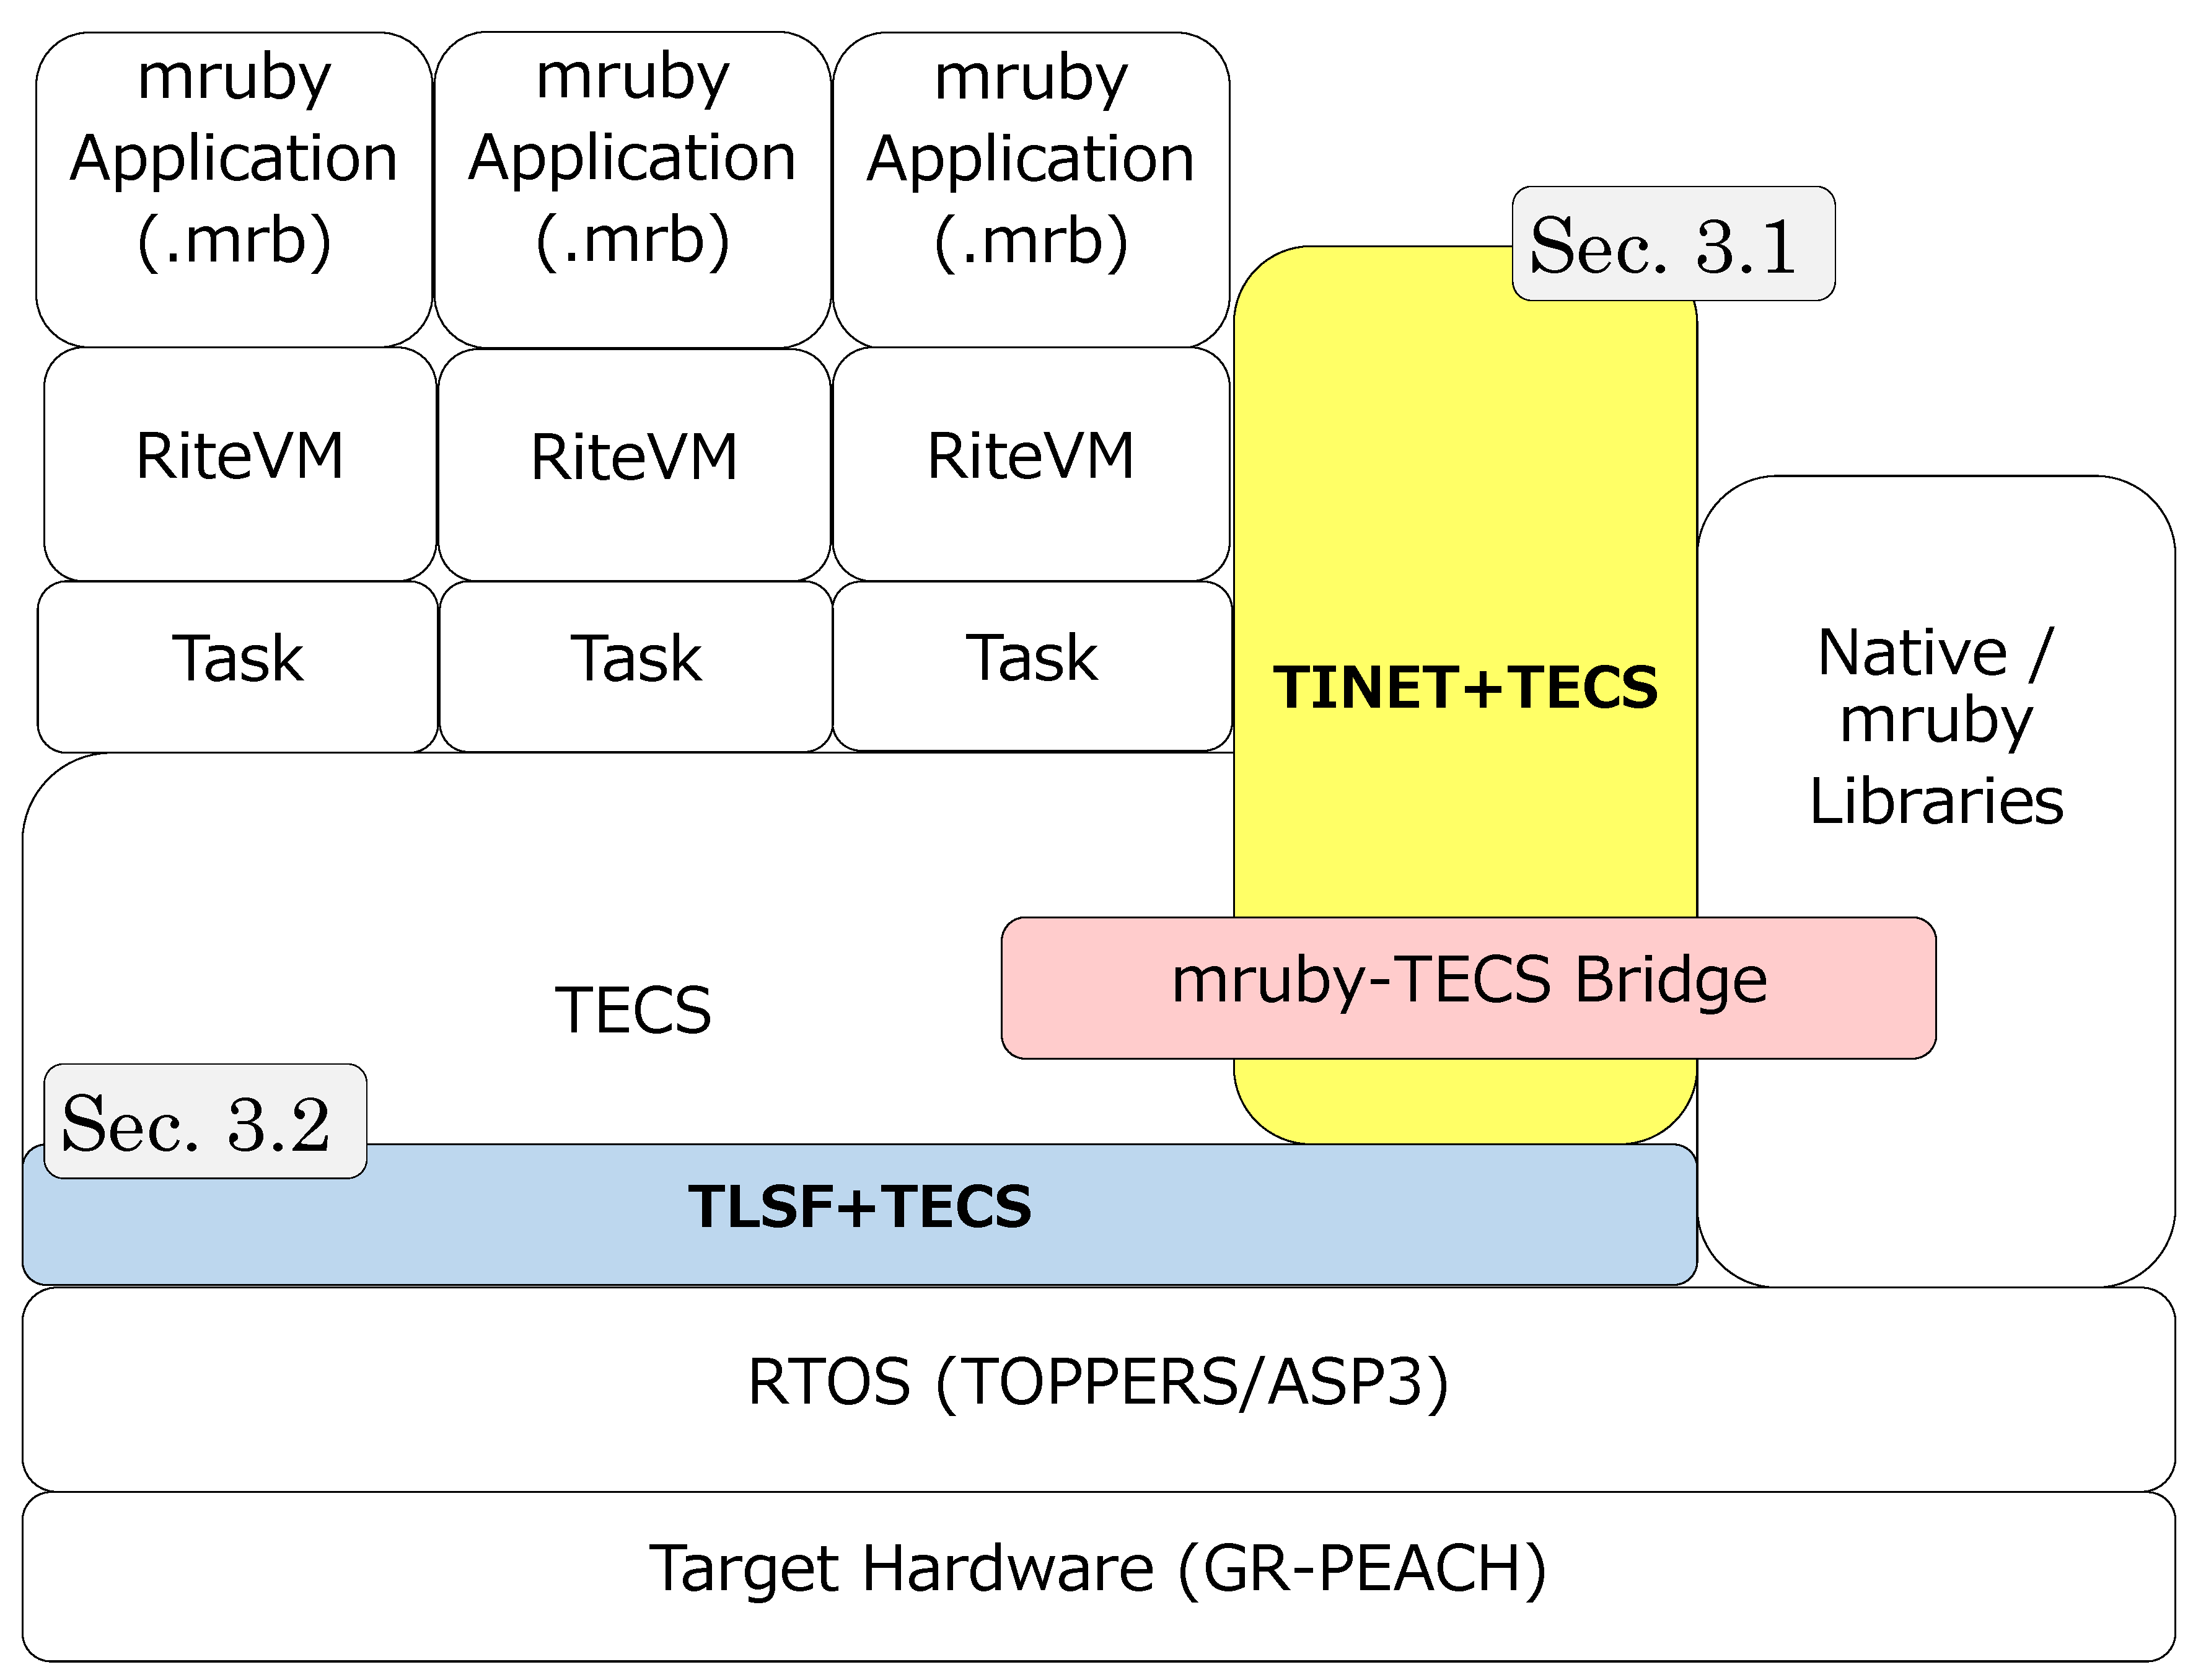
\includegraphics[width=8cm,clip]{figure/SystemModel.pdf}
    \caption{System model of the proposed framework}
    \label{fig:SystemModel}
\end{figure}

\subsection{TECS}
\label{sec:TECS}

TECS is a component system suitable for embedded systems.
TECS can increase productivity and reduce development costs due to improved reusability of software components.
TECS also provides component diagrams, which help developers visualize the overall structure of a system.

TECS statically performs component deployment and composition.
Consequently, connecting components does not incur significant overheads and memory requirements can be reduced.
TECS can be implemented in C, and demonstrates various features such as source level portability and fine-grained components.

\begin{figure}[t]
    \centering
    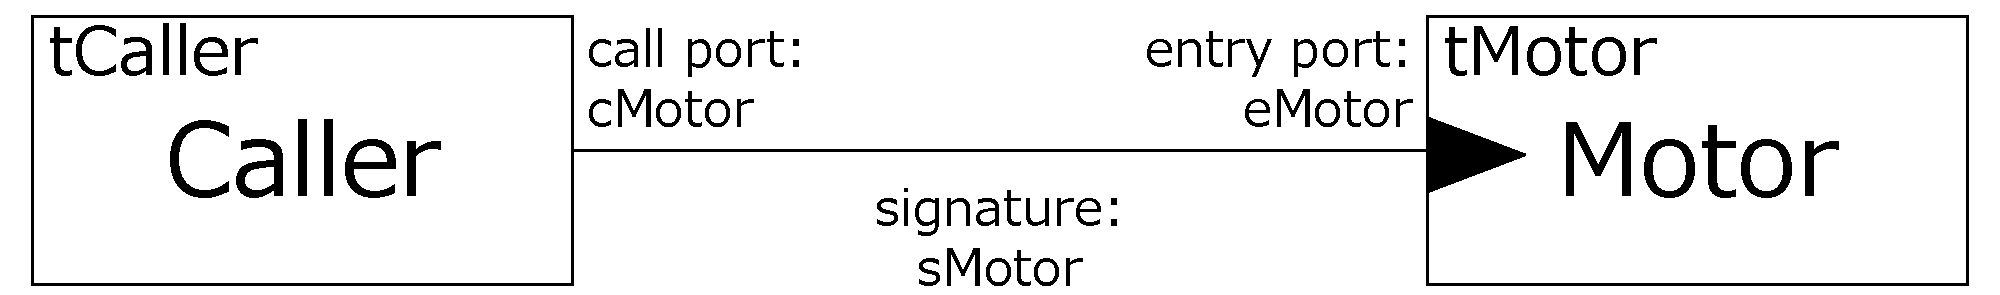
\includegraphics[width=8cm,clip]{figure/component_diagram.pdf}
    \caption{Component Diagram}
    \label{fig:component}
\end{figure}

\subsubsection{Component Model}
Fig.\ref{fig:component} shows a component diagram.
A {\it cell}, which is an instance of a TECS component, consists of {\it entry} ports, {\it call} ports, attributes and variables.
An {\it entry} port is an interface that provides functions to other {\it cell}s, and a {\it call} port is an interface that enables the use of other {\it cell}'s functions.
A {\it cell} has one or more {\it entry} ports and {\it call} ports.
{\it Cell} functions are implemented in C.

The type of {\it entry}/{\it call} port is defined by a {\it signature}, which is a set of functions.
A {\it signature} is the interface definition of a {\it cell}.
The {\it cell}'s  {\it call} port can be connected to the {\it entry} port of another {\it cell} by the same {\it signature}.
Here, {\it celltype} defines one or more {\it call}/{\it entry} ports, attributes, and internal variables of a {\it cell}.


\subsubsection{Component Description}
In TECS, components are described by {\it signature}, {\it celltype}, and build written in component description language (CDL).
These components are described as follows.

\begin{description}
    \item[{\bf Signature Description}]
        The {\it signature} defines a {\it cell} interface.
        The {\it signature} name follows the keyword {\it signature} and takes the prefix ``s'' e.g., sMotor (Fig.\ref{signature}).
        In TECS, to clarify the function of an interface, specifiers such as [in] and [out] are used, which represent input and output, respectively.
\begin{figure}[t]
\centering
\begin{lstlisting}
signature sMotor {
    void initializePort( [in]int32_t type );
    ER setPower( [in]int power );
    ER stop( [in] bool_t brake );
};
\end{lstlisting}
\caption{Signature Description}
\label{signature}
\end{figure}
    \item[{\bf Celltype Description}]
        The {\it celltype} defines {\it entry} ports, {\it call} ports, attributes, and variables.
        A {\it celltype} name with the prefix ``t'' follows the keyword {\it celltype}, e.g., tCaller (Fig.\ref{celltype}).
        To define {\it entry} ports, a {\it signature}, e.g., sMotor, and an {\it entry} port name, e.g., eMotor, follow the keyword {\it entry}.
        {\it Call} ports are defined similarly.
        Attributes and variables follow the keywords {\it attr} and {\it var}, respectively.
\begin{figure}[t]
\centering
\begin{lstlisting}
celltype tCaller {
    call sMotor cMotor;
};
celltype tMotor {
    entry sMotor eMotor;
    attr { int32_t port; };
    var { int32_t currentSpeed = 0; };
};
\end{lstlisting}
\caption{Celltype Description}
\label{celltype}
\end{figure}
    \item[{\bf Build Description}]
        The build description is used to instantiate and connect {\it cell}s.
        Fig.\ref{build} shows an example of a build description.
        A {\it celltype} name and {\it cell} name, e.g., tMotor and Motor, respectively, follow the keyword {\it cell}.
        To compose {\it cell}s, a {\it call} port, {\it cell}'s name, and an {\it entry} port are described in that order.
        In Fig.\ref{build}, {\it entry} port eMotor in {\it cell} Motor is connected to {\it call} port cMotor in {\it cell} Caller.
        {\it C\_EXP} calls macros defined in C files.

\begin{figure}[t]
\centering
\begin{lstlisting}
cell tMotor Motor {
    port = C_EXP("PORT_A");
};
cell tCaller Caller {
    cMotor = Motor.eMotor;
};
\end{lstlisting}
\caption{Build Description}
\label{build}
\end{figure}

\end{description}

\subsubsection{Development Flow}

\begin{figure}[t]
    \centering
    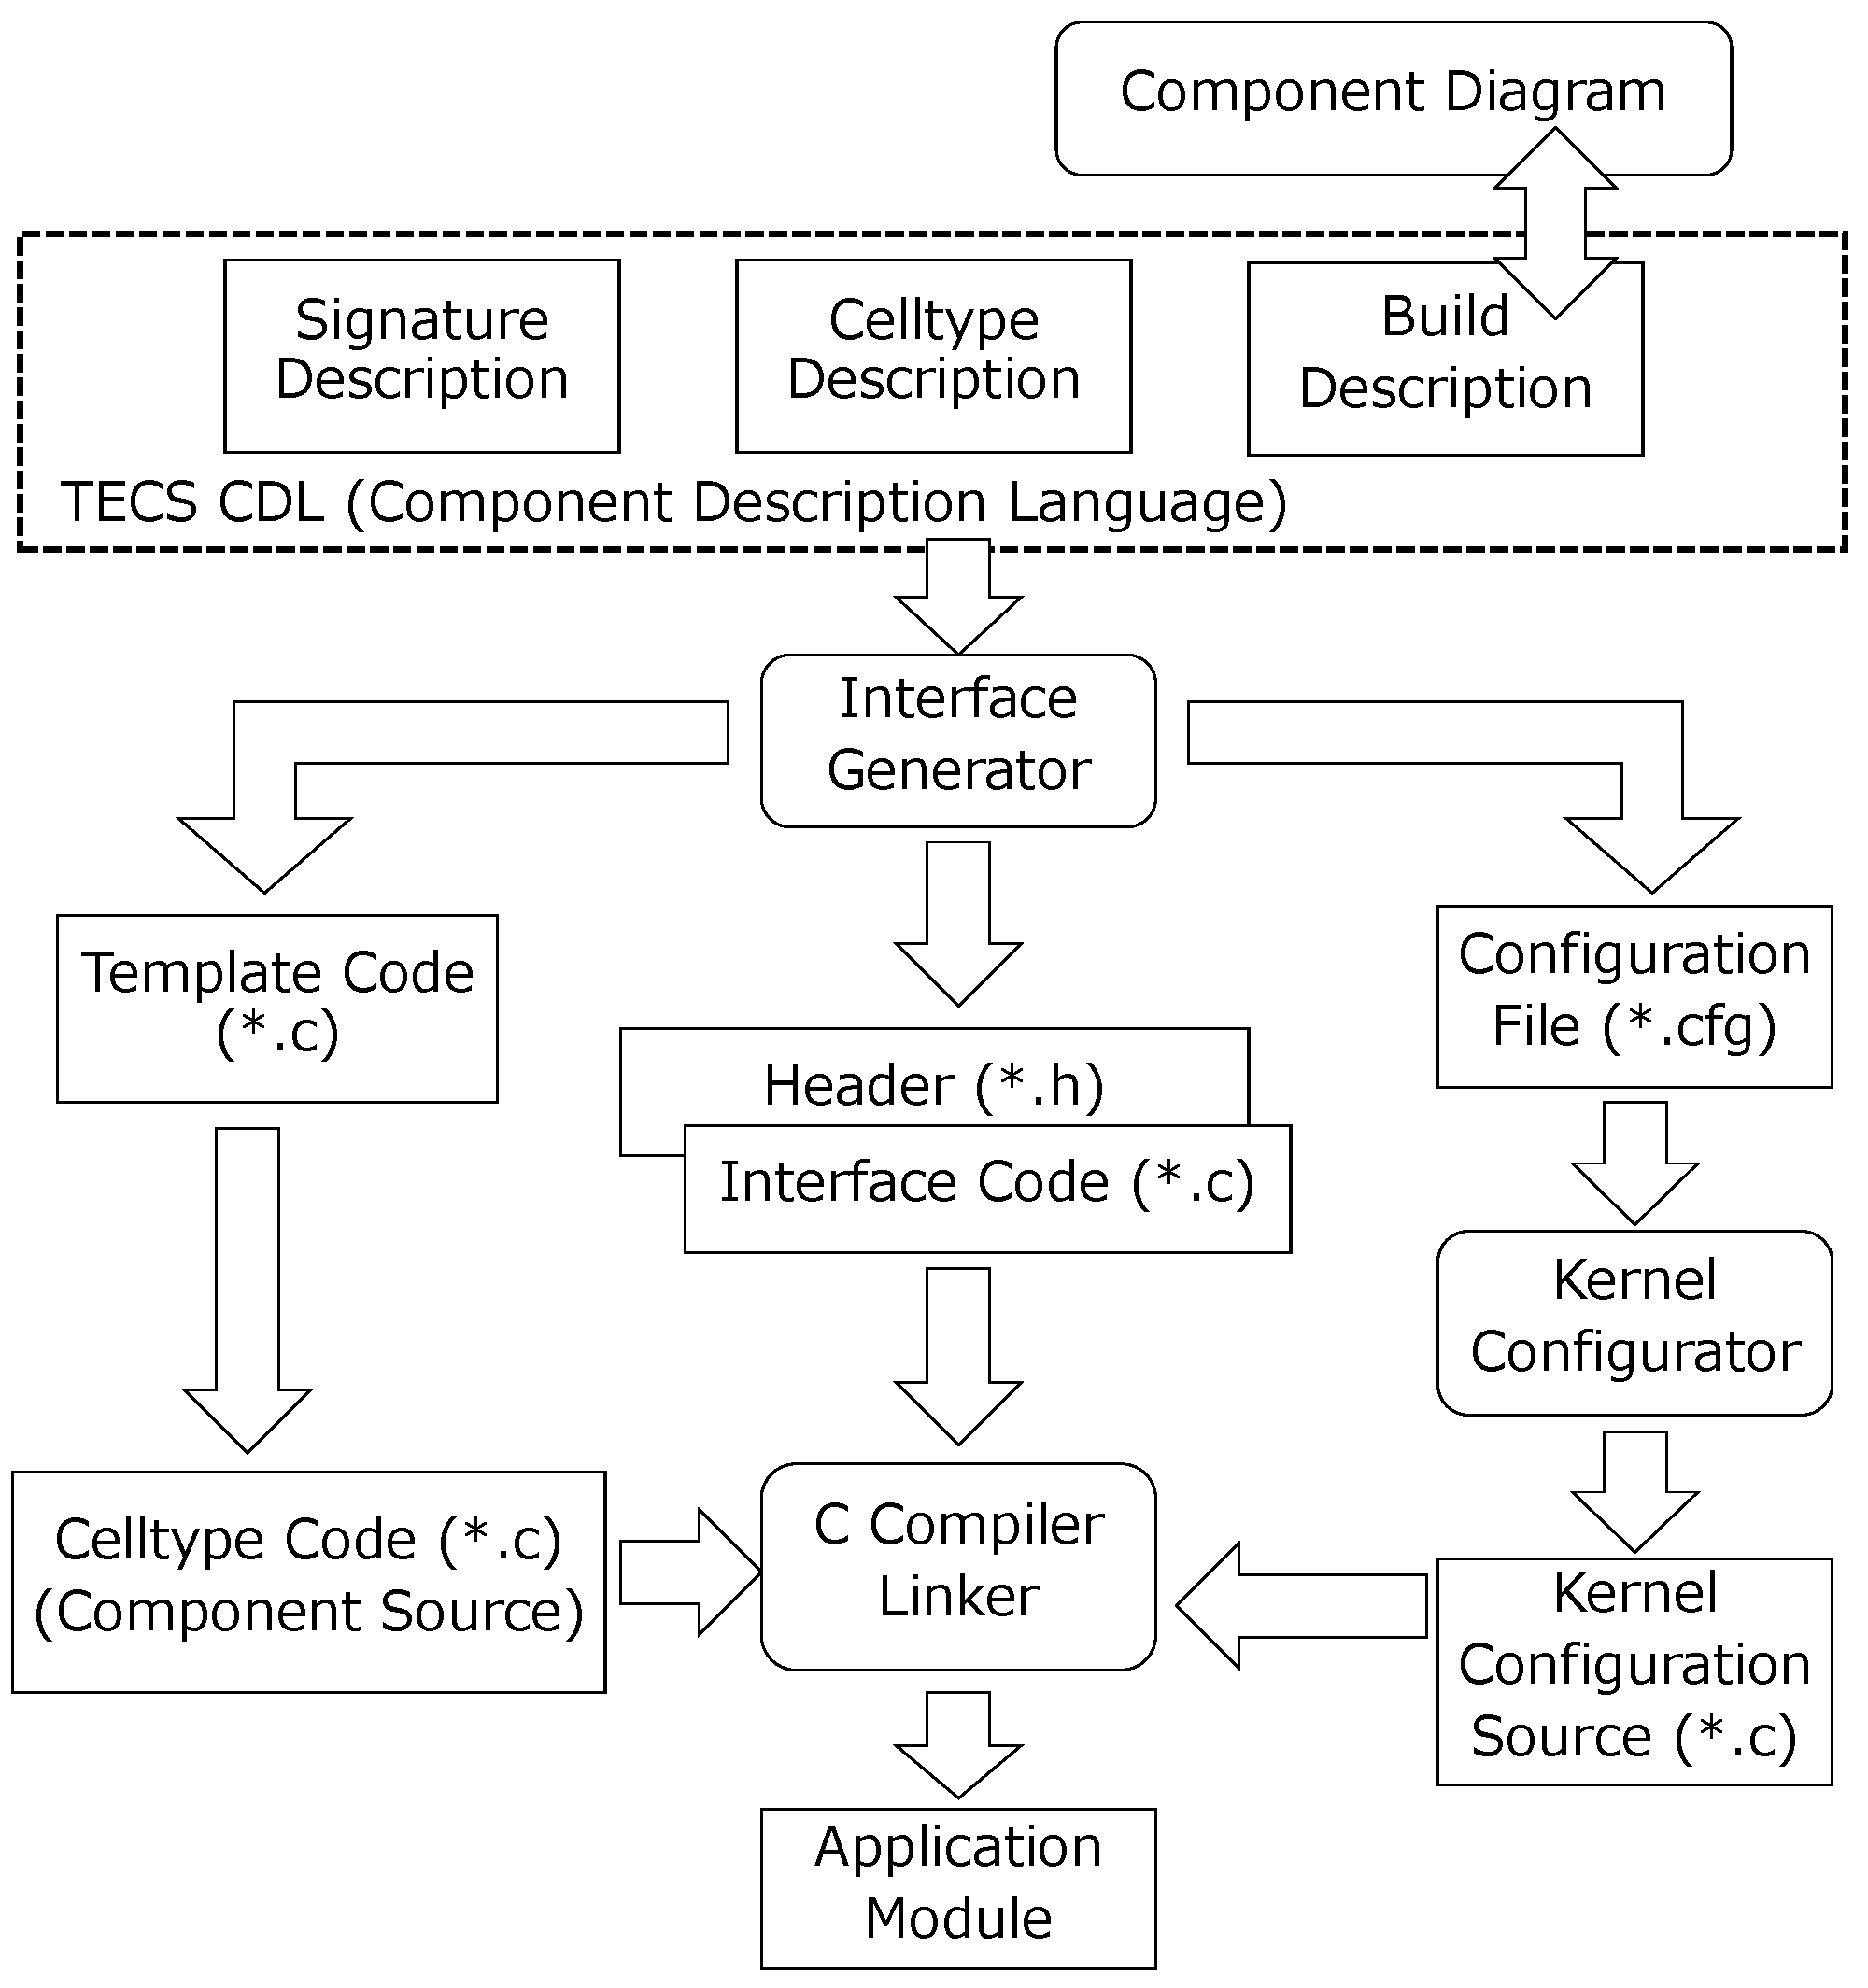
\includegraphics[width=8cm,clip]{figure/TECSFlow.pdf}
    \caption{Development flow using TECS}
    \label{fig:TECSFlow}
\end{figure}

Fig.\ref{fig:TECSFlow} shows the development flow using TECS.
TECS generator generates the interface code (.H and .C) and the configure file of the RTOS (.cfg) from the CDL file.

Software developers using TECS can be divided into component designers and application developers.
Component designers define {\it signature}s, which are interfaces between {\it cell}s, and {\it celltype}s, which are types of {\it cell}s.
Using the template code generated from the CDL file in which these are defined, component designers implement the functions and behaviors of the component in C language.
The source code implementing the function of the component is called a {\it celltype} code.
Application developers develop applications by using component diagrams and predefined {\it celltype} to connect {\it cell}s with build description.
An application module is generated by compiling and linking the header, the interface code, and the {\it celltype} code.


\subsection{mruby}
\label{sec:mruby}

mruby is a light-weight implementation of the Ruby programming language complying to part of the ISO standard \cite{url:mruby}.
Ruby is an object-oriented scripting language \cite{url:Ruby} with classes and methods, exceptions, and garbage collection functions.
It is easy to use and read due to its simple grammar and Ruby requires fewer lines of code than C.
Ruby improves the productivity of software development due to its simple grammar and object-oriented functions.

mruby, which retains the usability and readability of Ruby, requires fewer resources, and thus, is suitable for embedded systems.
In addition, mruby includes a VM mechanism, and thus, mruby programs can run on any operating system as long as a VM is implemented.
The mruby/RiteVM mechanism is shown in Fig.\ref{fig:mruby}.
The mruby compiler translates an mruby code into a bytecode, which can be interpreted by a RiteVM; thus, mruby programs can be executed on any target device with a RiteVM.

\begin{figure}[t]
    \centering
    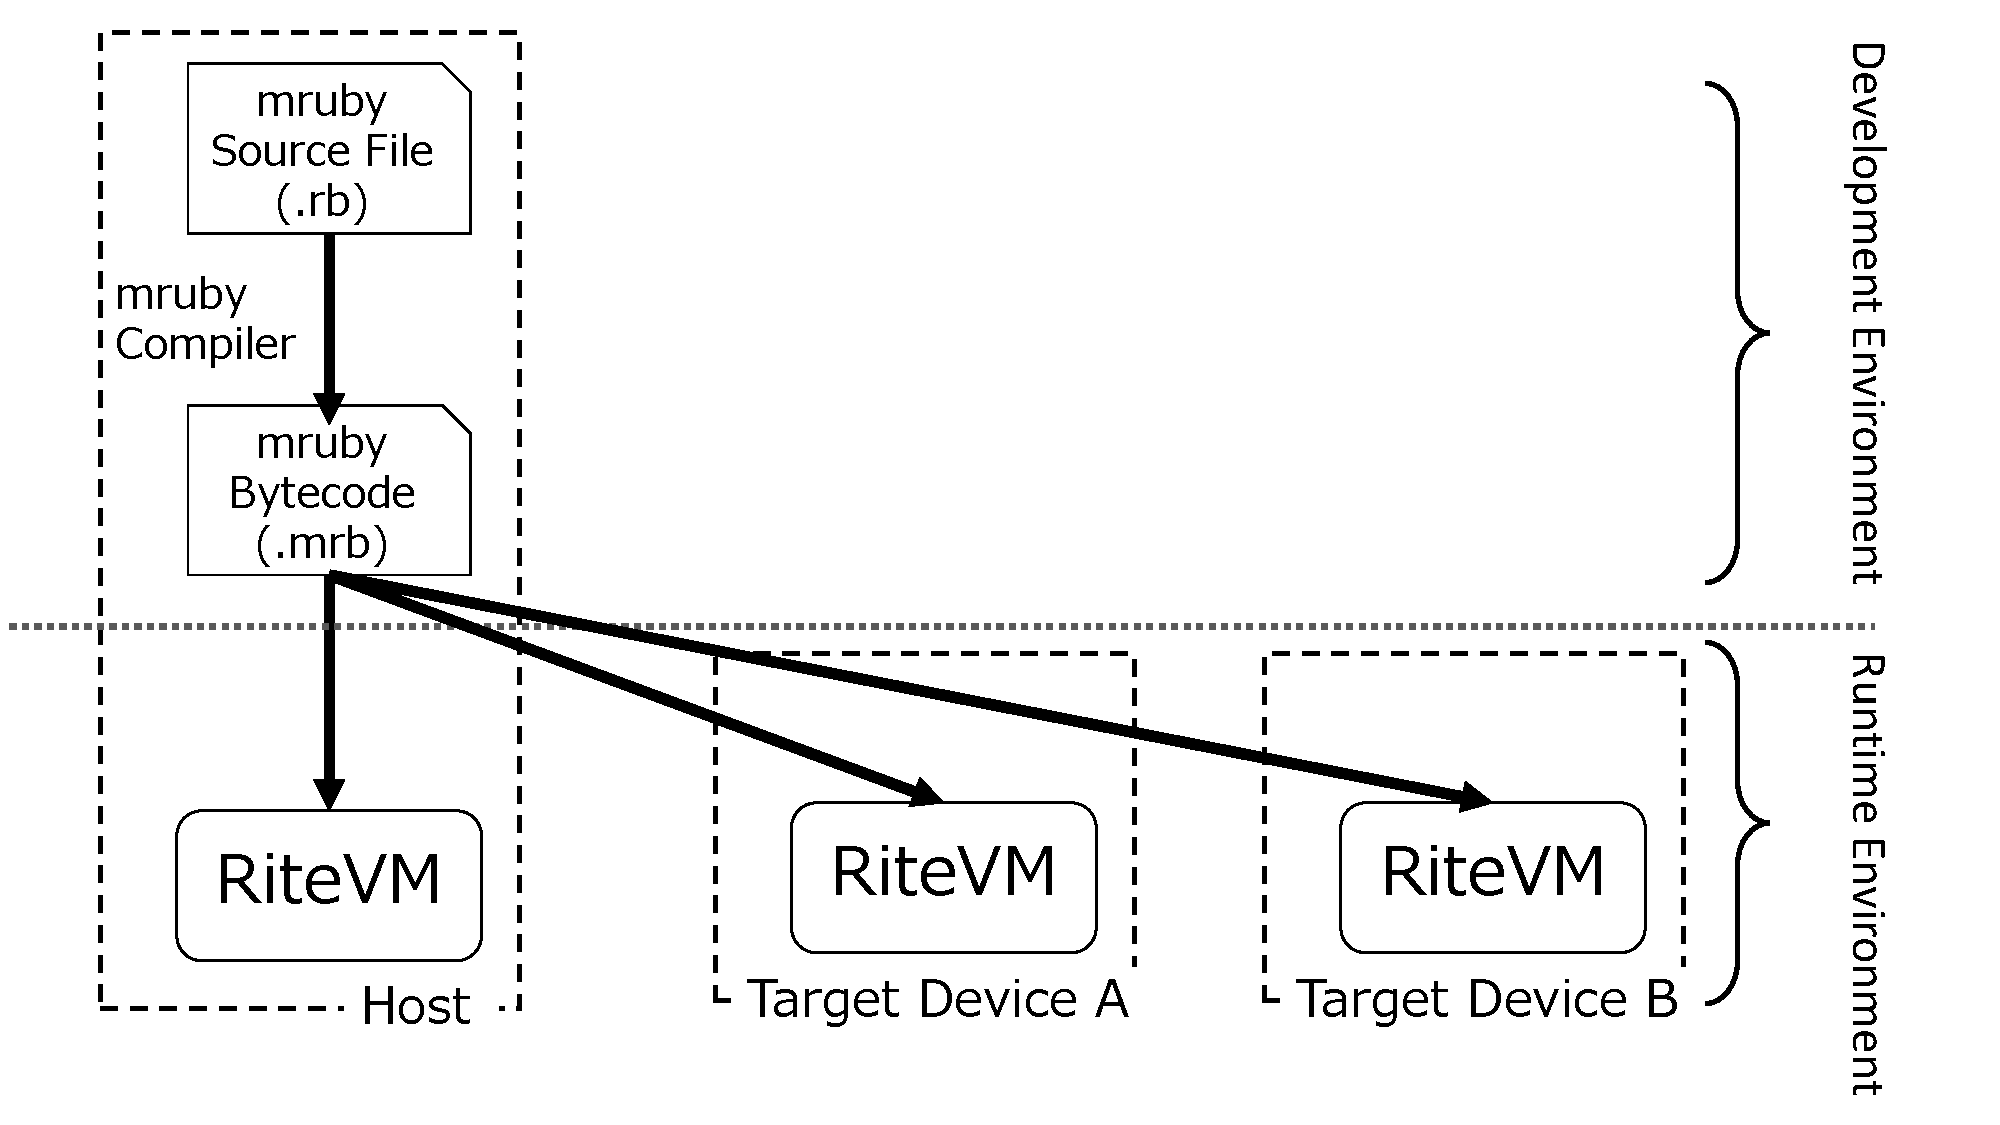
\includegraphics[width=8cm,clip]{figure/mruby.pdf}
    \caption{mruby/RiteVM mechanism}
    \label{fig:mruby}
\end{figure}


\subsection{mruby on TECS}
\label{sec:mrubyonTECS}

mruby on TECS is a component-based framework for running an mruby script language on embedded systems.
This framework integrates two technologies, mruby and TECS, and enables the development of embedded software using a script language without slowing down the execution time. 

\subsubsection{System Model of mruby on TECS}
% The present mruby on TECS system model is shown in Fig.\ref{fig:mrubyonTECS}.
Each mruby program, which is a bytecode, runs on its own RiteVM as a componentized task of an RTOS.
TECS components support various embedded drivers such as motor and sensor drivers.
An mruby-TECS bridge provides native libraries for mruby and can call a native program (e.g., C legacy code) from an mruby program.
The mruby-TECS bridge also provides TECS components for receiving the invocation from an mruby program.

In this paper, TOPPERS/ASP3 \cite{par:ASP3},\cite{url:ASP3} is the target RTOS and is based on $\mu$ITRON \cite{par:microITRON} .
However, mruby on TECS does not depend on the RTOS because TECS supports not only TOPPERS/ASP3 but also the other RTOSs such as OSEK \cite{par:OSEK} and TOPPERS/HRP2 \cite{url:HRP2},\cite{par:hr-tecs}.

% \begin{figure}[t]
%     \centering
%     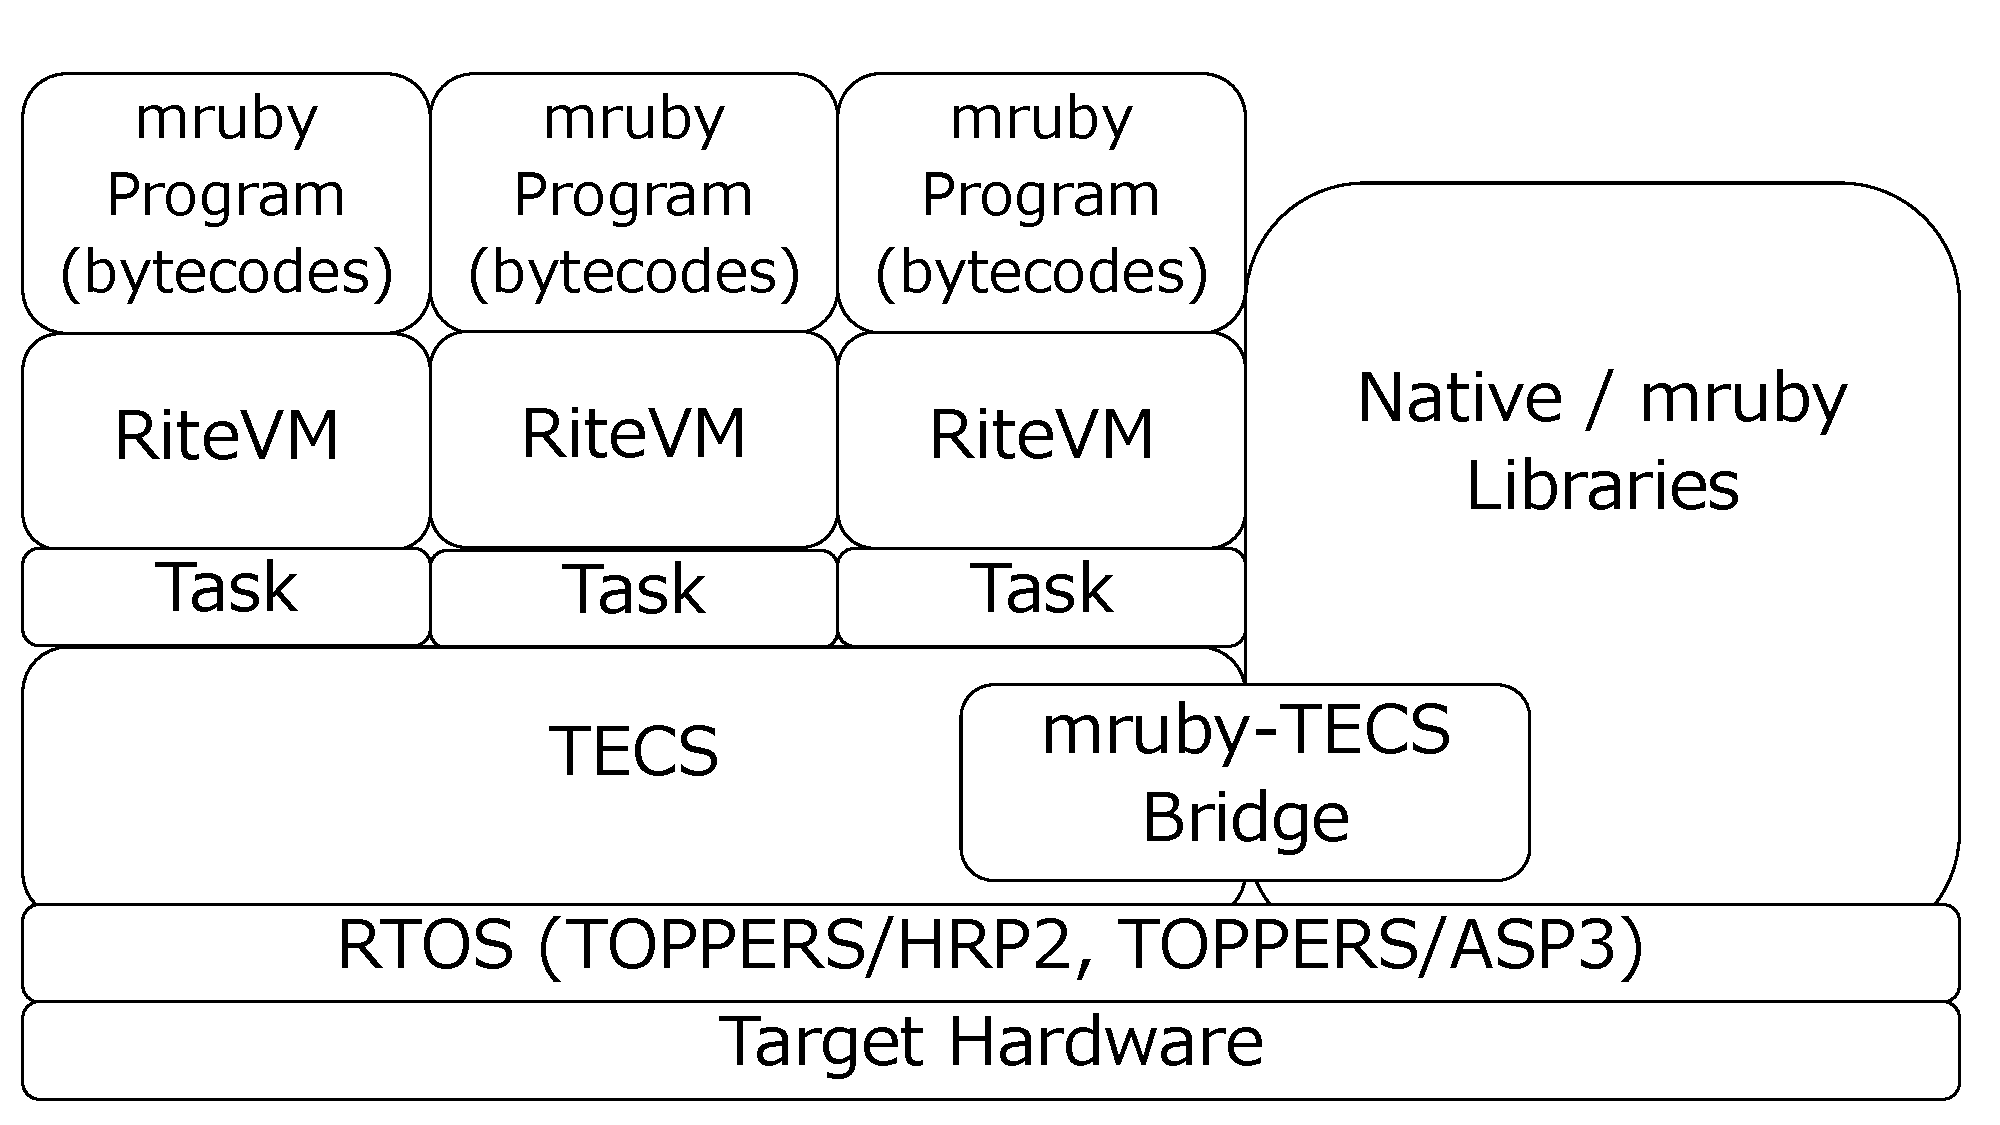
\includegraphics[width=6.5cm,clip]{figure/mrubyonTECS.pdf}
% \caption{System model of existing mruby on TECS}
% \label{fig:mrubyonTECS}
% \end{figure}

\subsubsection{mruby-TECS Bridge}
There is a significant difference between the execution times of mruby and C language codes.
According to  \cite{par:mrubyonTECS}, mruby programs are several hundred times slower than C programs and the execution of an mruby bytecode on a RiteVM is not as efficient as that of C code.
Thus, it is difficult to use mruby exclusively.

Using Ruby on embedded devices improves productivity and maintainability because it is easy to use and read.
However, some C language codes are required to manipulate actuators and sensors and ensure that critical sections of the code run quickly.

Fig.\ref{fig:mrubyTECSbridge} illustrates an mruby-TECS bridge used to control a motor.
The left side of BridgeMotor belongs to the mruby program.
The right side of BridgeMotor belongs to the TECS component.

\begin{figure}[t]
    \centering
    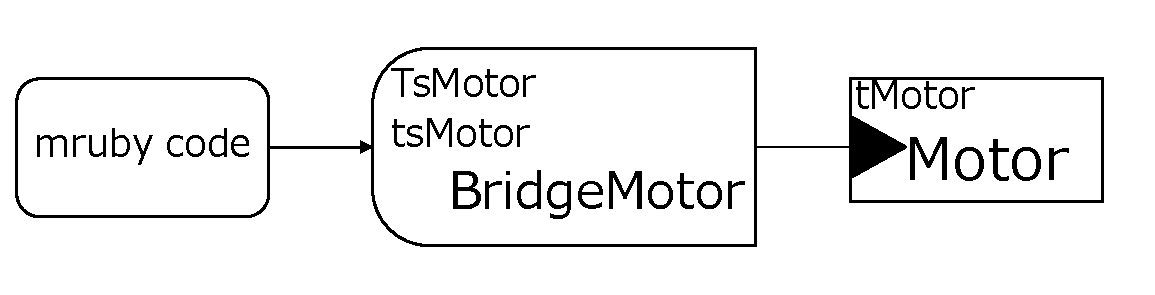
\includegraphics[width=8cm,clip]{figure/mrubyTECSbridge.pdf}
\caption{mruby-TECS bridge}
\label{fig:mrubyTECSbridge}
\end{figure}

The mruby-TECS bridge generates a {\it celltype}, which is called from the mruby code, and an mruby class, which corresponds to a developer-specified TECS component to invoke a C function from the mruby program.
The generated mruby-TECS bridge supports the registration of classes and methods for mruby.
Methods in an mruby class are defined by generation codes for an mruby-TECS bridge, such as setPower and stop.
Thus, when a method is called in an mruby program, the mruby-TECS bridge calls the function defined in the TECS component such as a Motor {\it cell}.

%3
\section{Proposed Framework}
\label{sec:Proposed Framework}

The proposed framework is an extended mruby on TECS framework to develop network software for IoT devices.
Developers can use TCP- and UDP-related functions from mruby programs.
The proposed framework incorporates two functionalities: TINET+TECS and TLSF+TECS.
TINET+TECS is a component-based TCP/IP protocol stack comprised in the proposed framework, and it compensates for the original TINET's weak point that it is hard to maintain, extend, and analyze the software due to many complex source codes and improves the configurability.
TLSF+TECS which is a component-based dynamic memory allocator is used for the memory management of RiteVMs and TCP/IP buffers in the proposed framework.
Since each TLSF component maintains its own heap area, TLSF+TECS allows concurrent operation without exclusive control while improving the efficiency of memory consumption, which is the advantage of TLSF.


\subsection{TINET+TECS}
\label{sec:TINET+TECS}

\subsubsection{TINET}

TINET is a compact TCP/IP protocol stack for embedded systems based on the ITRON\footnote{ITRON is an RTOS developed by the TRON project.} TCP/IP API Specification \cite{url:ITRON_TCP/IP_API_Spec}, developed by the TOPPERS Project \cite{url:TOPPERS}.
TINET has been released as an open-source tool.
To satisfy restrictions for embedded systems in terms of, for example, memory capacity, size, and power consumption, TINET supports functions such as minimum copy frequency, elimination of dynamic memory control, asynchronous interfacing, error detailing per API.

{\bf Overview:}
TINET runs as middleware on TOPPERS/ASP3 \cite{par:ASP3} \cite{url:ASP3}, a real-time kernel based on $\mu$ITRON \cite{par:microITRON}.
As it is compatible with TOPPERS RTOS, TINET also supports other RTOSs such as TOPPERS/ASP and TOPPERS/JSP.

Fig.\ref{fig:TINETHierarchyDiagram} shows the hierarchy diagram of TINET and TOPPERS/ASP3.
Users send and receive data using a Communication End Point (CEP), an interface that functions like a socket.
In the transmission process, headers are attached to the data body passed to the CEP at each protocol layer before the data are transmitted from the network device.
In the reception process, the headers of the data bodies received by the network device are analyzed at each protocol layer, and the data are then passed to the CEP.

A TCP reception point called the REP stands by to receive connection requests from the partner side.
The REP has an IP address ({\it myaddr}) and a port number ({\it myportno}) as attributes and performs functions such {\it bind()} and {\it listen()}.

In TINET, the amount of data copying at each protocol layer is minimized.
In standard computing systems, the TCP/IP protocol stack has large overheads in terms of execution time and memory consumption because the data are copied at each protocol layer.
To solve this problem, TINET does pass the pointer of the data buffer between each protocol layer instead of data copying.

\begin{figure}[t]
    \centering
    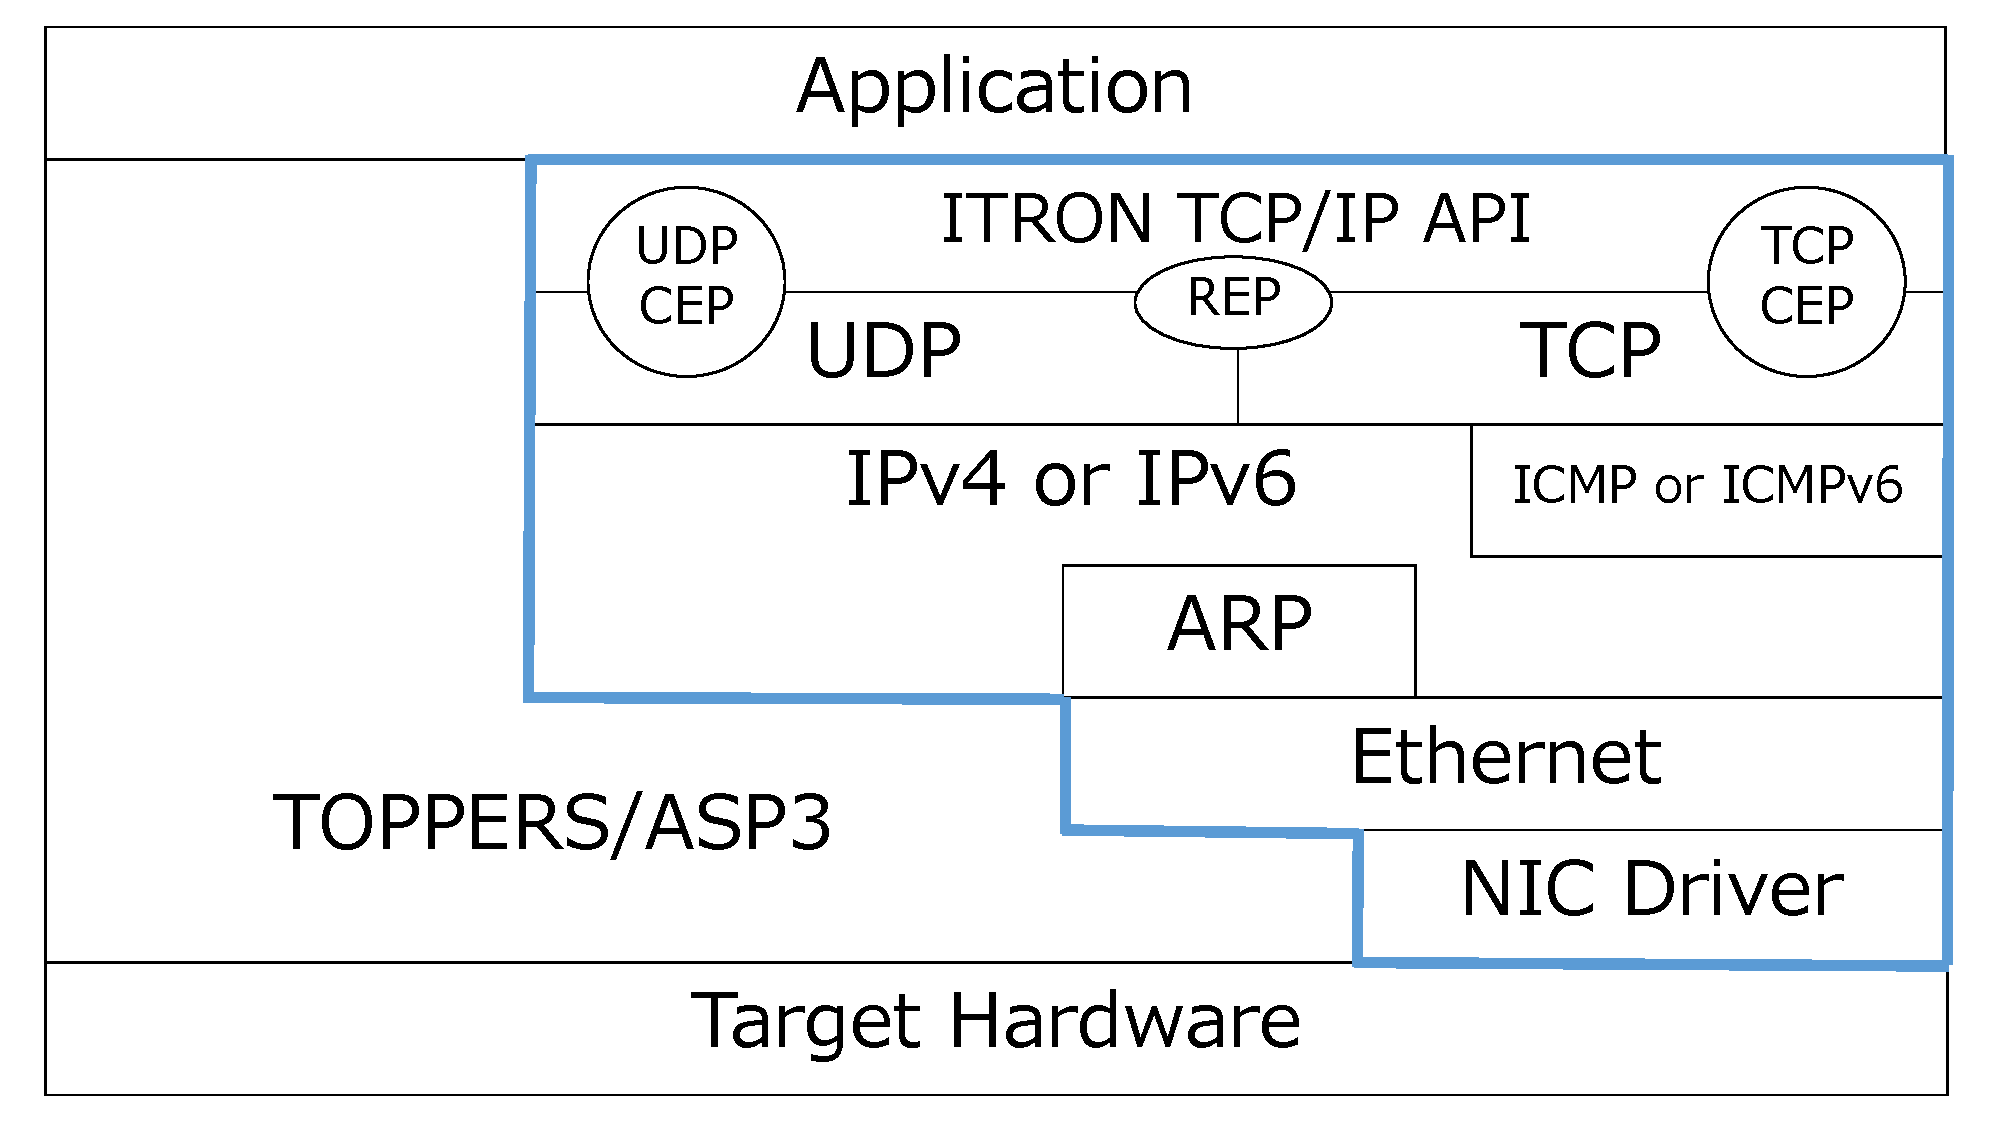
\includegraphics[width=8cm,clip]{figure/TINETHierarchyDiagram.pdf}
    \caption{TINET and TOPPERS/ASP3 hierarchy diagrams}
    \label{fig:TINETHierarchyDiagram}
\end{figure}

\subsubsection{Component Design of TINET+TECS}

TINET+TECS, the proposed componentized TCP/IP protocol stack, comprises a number of some TECS components.
This section describes the components of the TINET+TECS framework with the aid of component diagrams.

\subsubsection*{Components of a protocol stack}

The components of the TINET+TECS protocol stack are shown in Fig.\ref{fig:ComponentProtocolStack}.
Note that some small particle components, such as a kernel object, data queues, and semaphores, are omitted to simplify the component diagram.
In TINET+TECS, the components are divided for each protocol, and functionalities such as input/output functions are defined as respective components.
By using such small grain components, software visibility is improved.
The components of each protocol are described as follows.

\begin{figure}[t]
    \centering
    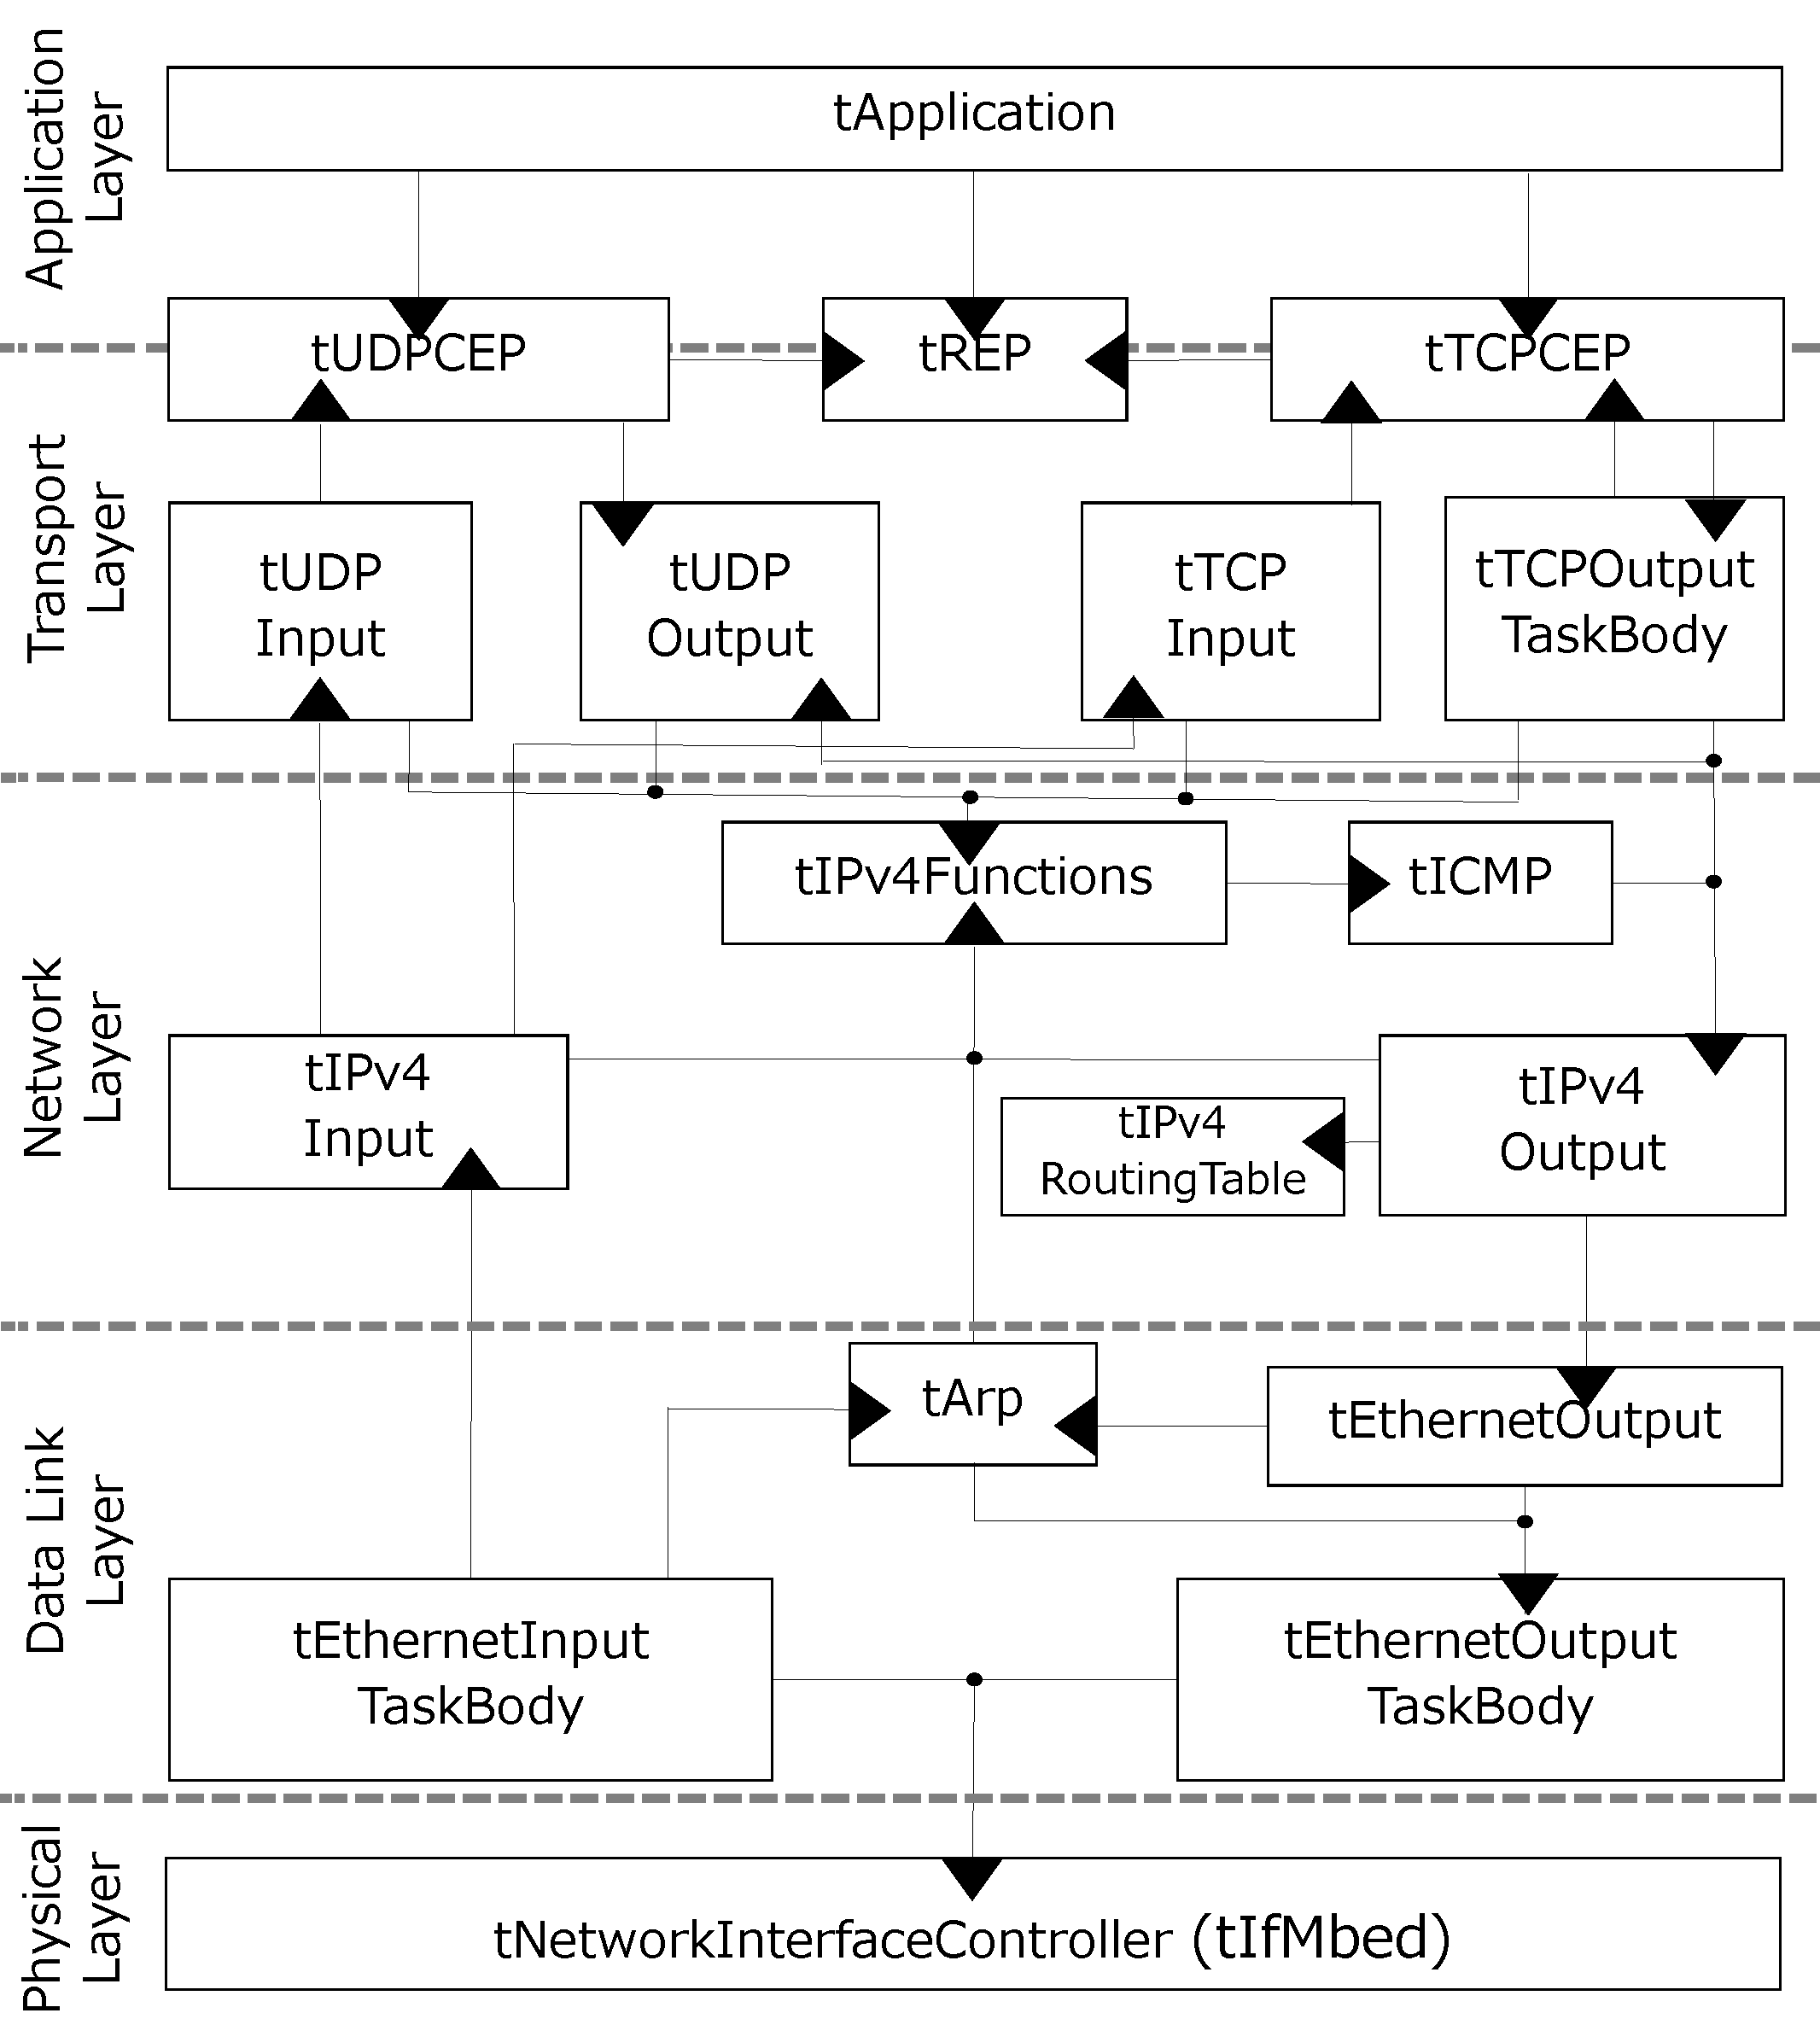
\includegraphics[width=8.0cm,clip]{figure/ComponentProtocolStack.pdf}
    \caption{Component diagram of a protocol stack}
    \label{fig:ComponentProtocolStack}
\end{figure}


{\bf Application layer:}
An application in TINET+TECS is implemented as a component such as tApplication.
Software with TINET uses ITRON TCP/IP API \cite{url:ITRON_TCP/IP_API_Spec} such as {\it tcp\_snd\_dat} and {\it tcp\_rcv\_dat}.
In TINET+TECS, the application component calls TECS functions such as {\it cTCPAPI\_sendData} and {\it cTCPAPI\_receiveData}.
Moreover, in TINET+TECS supporting a TECS adapter, an existing application with TINET can run on the TINET+TECS framework without transporting, and therefore, software can be developed either using existing methods or as TECS components.

{\bf Transport layer:}
tTCPCEP (tUDPCEP) and tREP are, respectively, CEP and REP components.
For example, a server program supporting multiple clients can be developed by preparing multiple tTCPCEP components.
tTCPInput and tTCPOutput are components for performing, respectively, receiving and sending processing in the transport layer.

{\bf Network layer:}
The tIPv4Input and tIPv4Output components perform, respectively, the receiving and sending processing in the network layer.
The tIPv4Functions component performs functions such as checksum, the tICMP component is used for the Internet Control Message Protocol (ICMP), and the tIPv4RoutingTable component operates a routing table.

{\bf Data link layer:}
tEthernetInputTaskBody and tEthernetOutputTaskBody (tEthernetOutput) are components for performing, respectively, receiving and sending processing in the data link layer.
The tArp component is for implementing the Address Resolution Protocol (ARP).

{\bf Physical layer:}
The tNetworkInterfaceContoroller component implements a network device driver.
Software can be run on other devices by replacing the component because only the component depends on the target device.

To utilize the protocol stack in the same manner in the original TINET, communication object components such as tTCPCEP, tUDPCEP, and tREP are defined as an interface between TINET+TECS and applications.
The communication object component corresponds to a CEP or REP of the original TINET.
Application developers can utilize TINET+TECS functionalities by generating and combining as many components as necessary.

TINET+TECS supports the coexistence of multiple protocols.
Though its use of IPv6 and Point-to-Point Protocol (PPP) components, TINET+TECS can make IPv4 and IPv6 coexist and support PPP without modification of component implementation.

\subsubsection*{Memory allocator component} 

The original TINET eliminates dynamic memory control to meet the severe memory restrictions of embedded systems.
A memory area for sending/receiving data in the protocol stack is allocated and released within a predetermined area.
The memory allocator component allows for the elimination of dynamic memory control in TINET+TECS by providing a requested memory area from the statically allocated memory area.

The memory allocator component connects to as many tFixedSizeMemoryPool as required, as shown in Fig.\ref{fig:tMemoryAllocator}.
tFixedSizeMemoryPool is a componentized kernel object of TOPPERS/ASP3 for allocating and releasing memory areas of a requested size. 
tFixedSizeMemoryPool components of various sizes are prepared, and an appropriate memory area can be allocated according to the used data size.
On the other hand, all components that need to allocate or deallocate memory, e.g., tTCPInput and tEthernetOutput, connect to the memory allocator component.

In addition, TINET+TECS utilizes the TECS {\it send/receive} specifier to minimize the memory copy frequency, which is a functionality supported by TINET.

\begin{figure}[t]
    \centering
    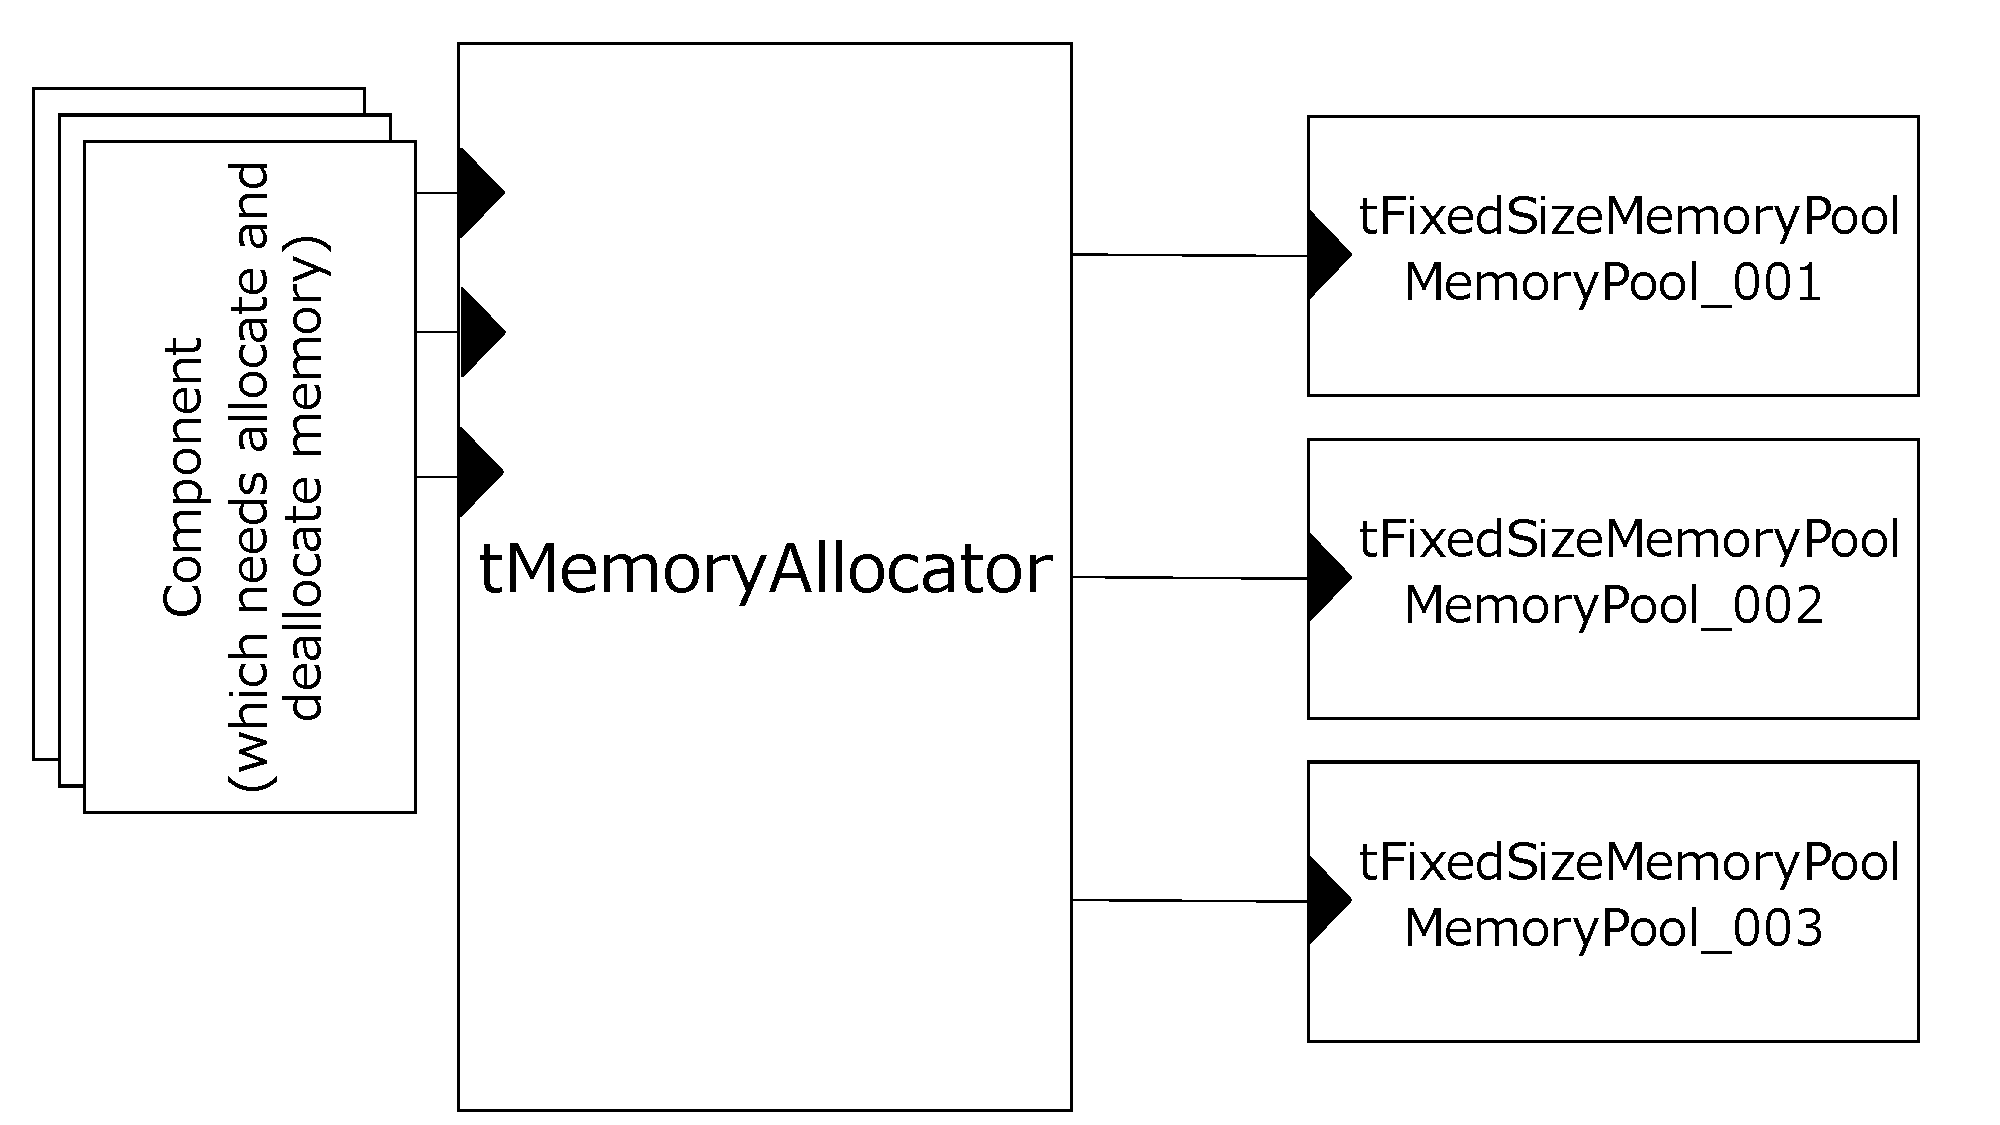
\includegraphics[width=8cm,clip]{figure/tMemoryAllocator.pdf}
    \caption{Component diagram of tMemoryAllocator}
    \label{fig:tMemoryAllocator}
\end{figure}

\begin{figure}[t]
    \centering
    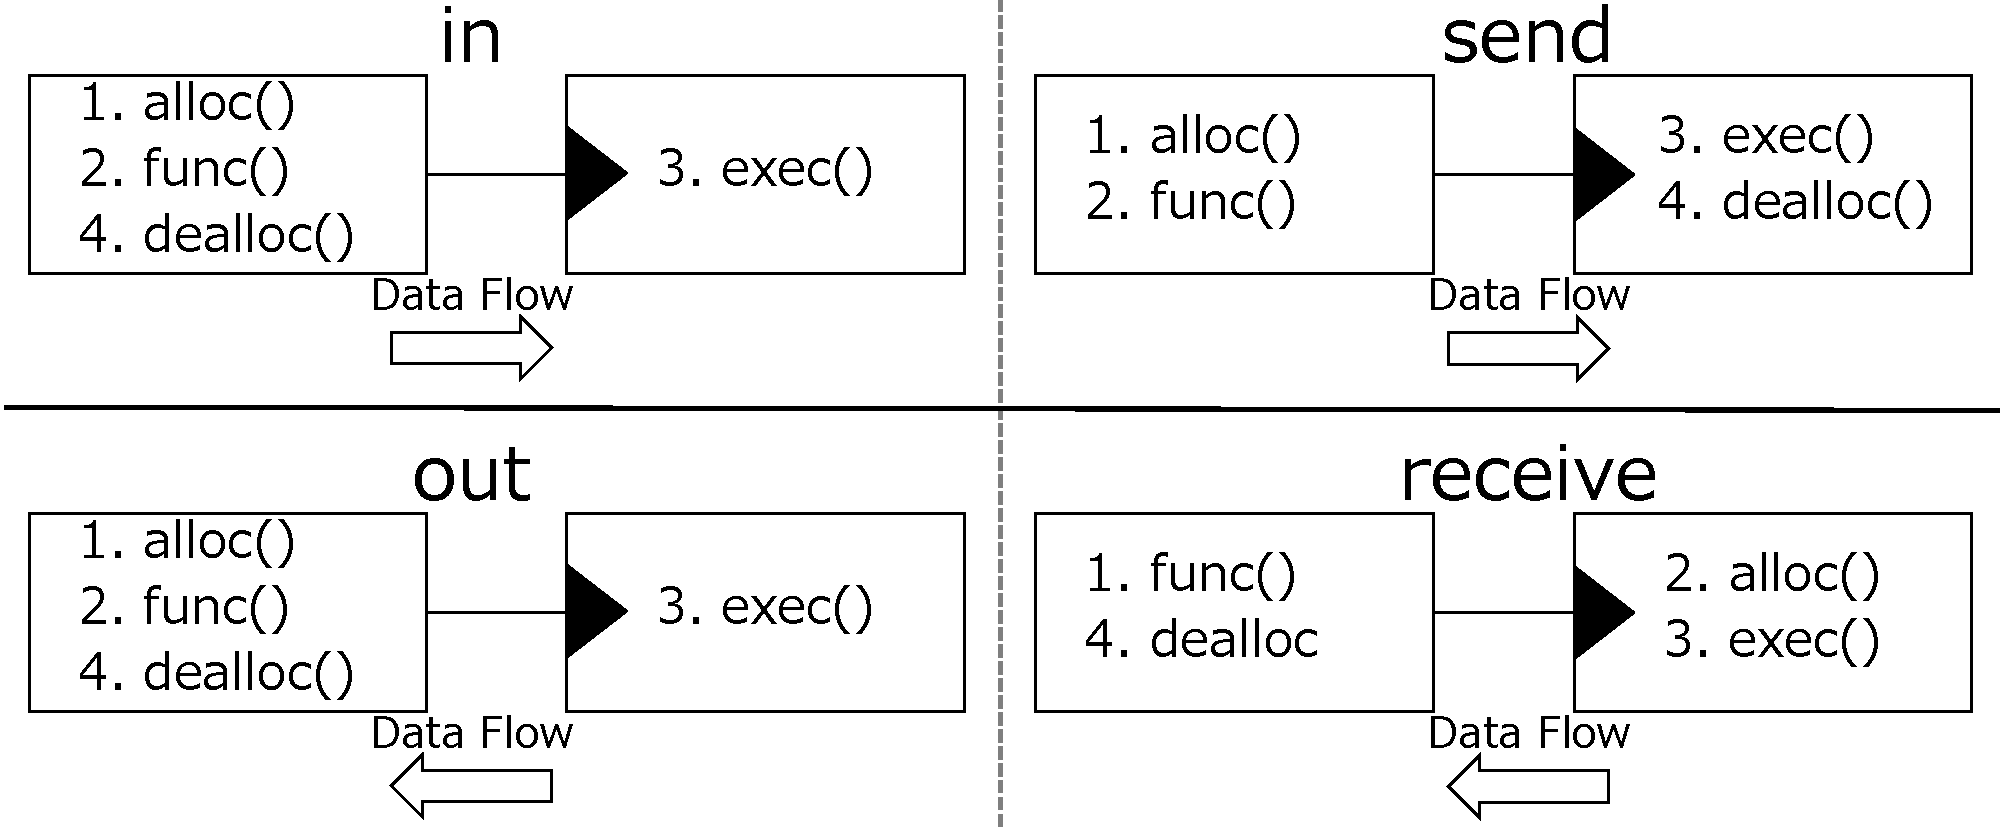
\includegraphics[width=8cm,clip]{figure/SendReceive.pdf}
    \caption{Differences between in/out and send/receive}
    \label{fig:SendReceive}
\end{figure}

{\bf Send/receive specifiers:}
TECS supports {\it send}/{\it receive} interface specifiers \cite{par:RPC}.
TINET+TECS uses {\it send} and {\it receive} specifiers instead of {\it in} and {\it out} to reduce the number of copies:

\begin{itemize}
\item {\it in} is a specifier for input arguments.
A callee side uses the memory of arguments with {\it in} when executing the callee function.
When the processing returns to the caller side, the caller can reuse and deallocate the memory.

\item {\it send} is another specifier for transferring data to a callee from a caller.
The difference between {\it in} and {\it send} is whether the data memory is deallocated in the caller or callee, as shown in Fig.\ref{fig:SendReceive}.
In the case of the {\it in} specifier, both allocating and deallocating of the data memory are performed in the caller.
By contrast, in the case of {\it send}, the caller allocates the data memory and the callee deallocates it.

\item {\it out} is a specifier for output arguments through which a callee writes data in the memory allocated by a caller while the caller receives the data.

\item {\it receive} is another specifier for a caller receiving data from a callee.
The difference between {\it out} and {\it receive} lies in whether the data memory is allocated in the caller or callee, as shown in Fig.\ref{fig:SendReceive}.
In the case of {\it out}, the callee writes data in the memory allocated by a caller, whereas in the {\it receive} case, the callee allocates the data memory.
Deallocating of the memory is performed in the caller in both cases.
\end{itemize}

As shown in Fig.\ref{src:SendReceive}, sending and receiving arguments such as {\it outputp} and {\it inputp} are defined using, respectively, the {\it send/receive} specifier in the signature description.
Developers hardly make mistakes of memory operation because these specifiers completely pass an ownership of memory.
Common object request broker architecture (CORBA) does not consider memory sharing; CORBA has no functionalities
such as {\it send}/{\it receive}.

\begin{figure}[t]
\centering
\begin{lstlisting}
signature sNicDriver {
  void start(
    [send(sNetworkAlloc),size_is(size)]
        int8_t *outputp, .., ..);
  void read(
    [receive(sNetworkAlloc),size_is(*size)]
        int8_t **inputp, .., ..);
    /* Omit: other functions */
};
\end{lstlisting}
\caption{Signature description of the nic driver (An example of send/receive)}
\label{src:SendReceive}
\end{figure}

\subsubsection{Dynamic connection in TECS}
\label{sec:DynamicConnection}

\begin{figure}[t]
    \centering
    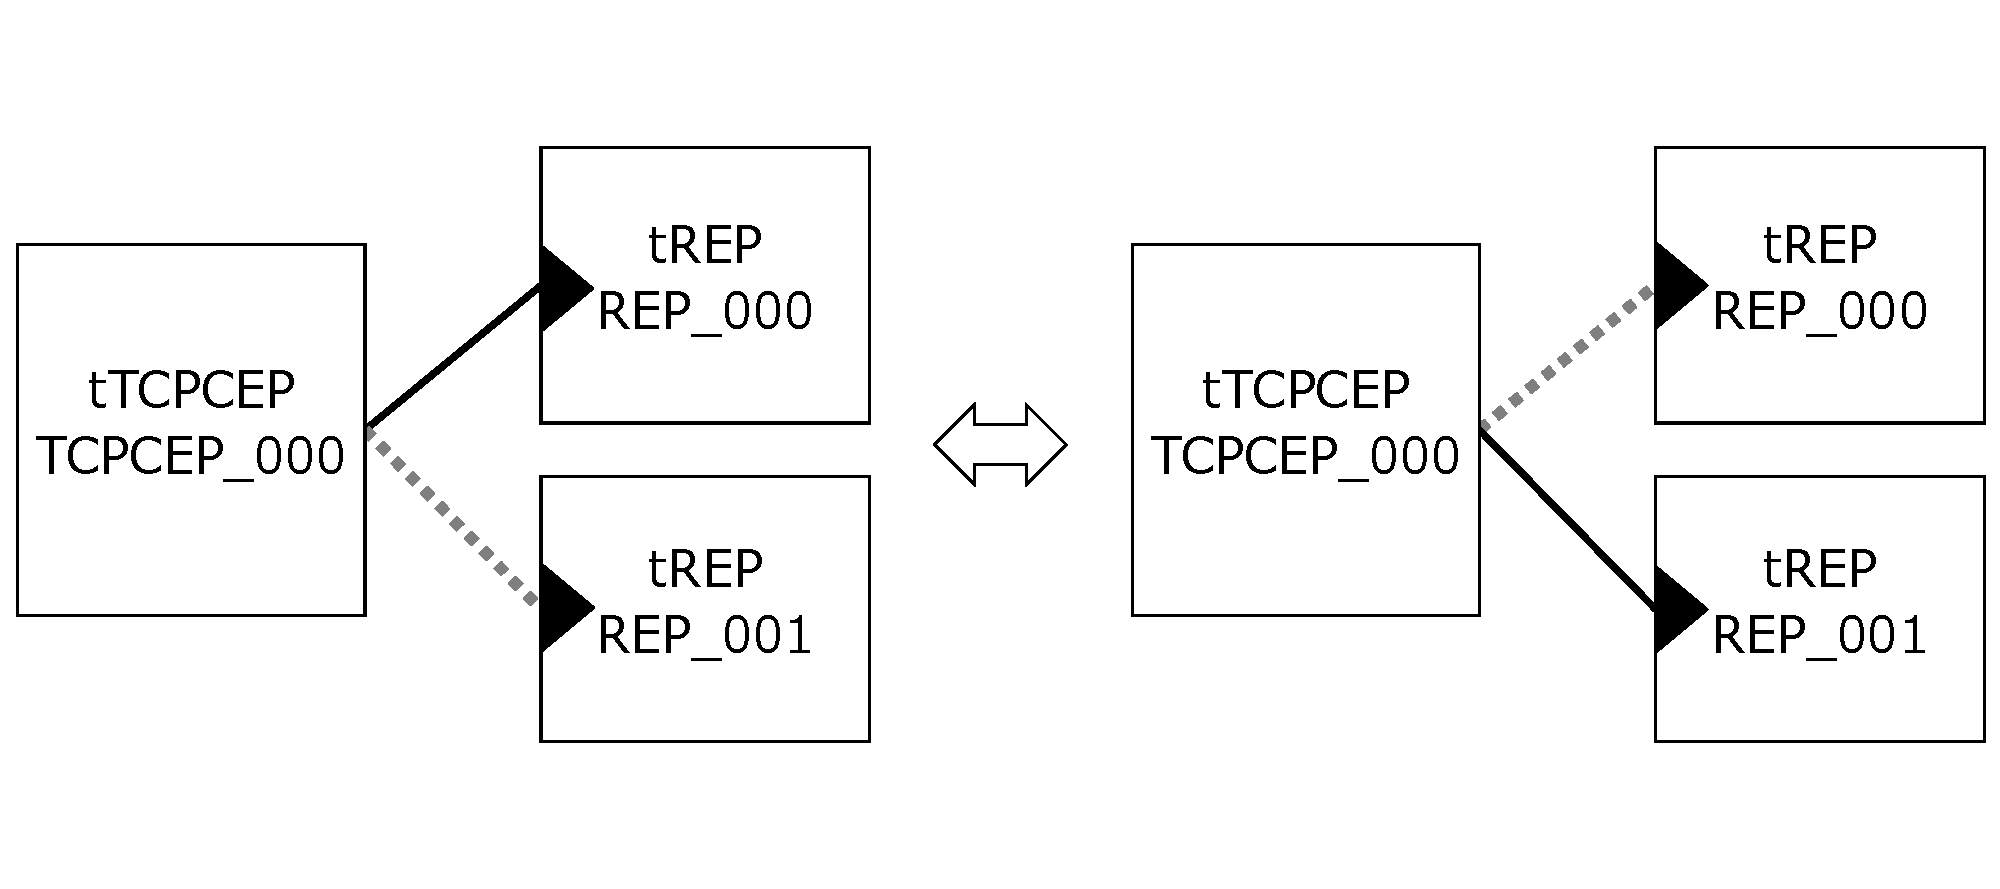
\includegraphics[width=8cm,clip]{figure/DynamicConnection.pdf}
    \caption{Dynamic connection}
    \label{fig:DynamicConnection}
\end{figure}

TECS supports a dynamic connection, a method for switching the binding of components at runtime (Fig.\ref{fig:DynamicConnection}) as a new functionality.
In Fig.\ref{fig:DynamicConnection}, the solid line represents binding and the dotted line represents non-binding.
Note that all components are statically generated in TECS, which can optimize the overhead of componentization because components are statically configured.
Dynamically generating components causes a good deal of memory consumption, which is a serious problem for embedded systems with strict memory constraints.
The proposed framework can take advantage of the componentization in TINET while satisfying the memory constraint because components are statically generated and dynamically connected in TECS.

TINET+TECS utilizes the dynamic connection to switch between CEP and REP components, as shown in Fig.\ref{fig:DynamicConnectionUseCase}.
In a server application, CEP is associated with REP in the state of waiting for a connection request from clients\footnote{tcp\_acp\_cep(ID cepid, ID repid, T\_IPV4EP *p\_dstaddr, TMO tmout).}.
For example, when processing with the HTTP protocol, CEP passively opens with an REP of port number 80.

\begin{figure}[t]
    \centering
    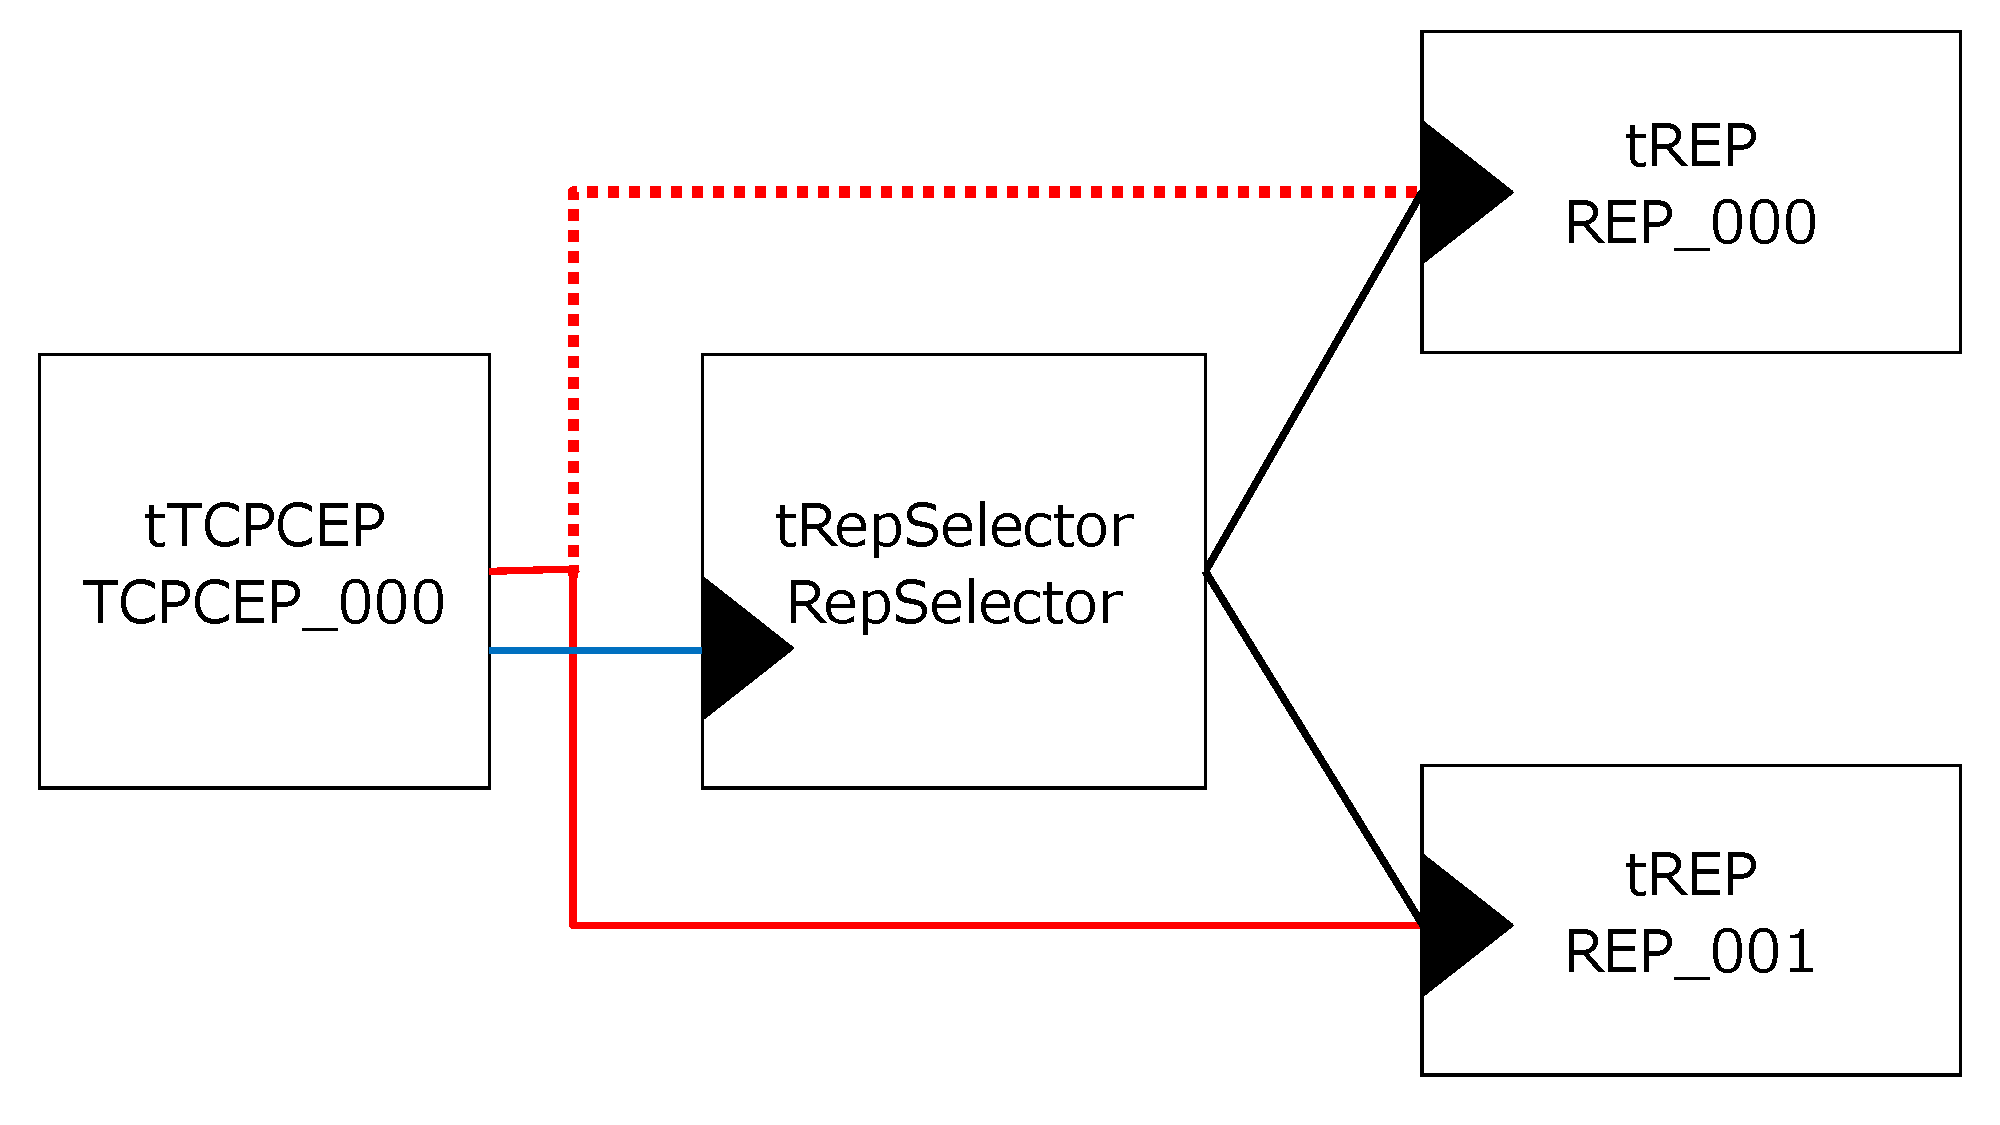
\includegraphics[width=8.0cm,clip]{figure/DynamicConnectionUseCase.pdf}
    \caption{Dynamic connection between CEP and REP}
    \label{fig:DynamicConnectionUseCase}
\end{figure}

To utilize dynamic connectivity, a selector should be defined.
A selector connects all components that can be dynamically connected under a common descriptor that serves as an identifier to access each component \cite{par:optimization}.
The cREP ports form a call port array connecting to connecting to all tREP cells (Line 8 in Fig.\ref{src:DynamicCDLcode}).
{\it [ref\_desc]} is used to identify call ports referring to descriptors. 
In the case of Fig.\ref{fig:DynamicConnectionUseCase}, the tRepSelector cell connects all tREP cells.

A CEP component has two call ports: the cRepSelector port, which connects to the eRepSelector port of tRepSelector cell, and the cREP4 port, which connects to either of the tREP cells (Lines 11--13 in Fig.\ref{src:DynamicCDLcode}).
The cREP port is defined using {\it [dynamic]} to identify the call port used to dynamically switch the components.
The call port with the {\it [dynamic]} specifier is not optimized and is allocated in RAM using a plug-in.

\begin{figure}[t]
\centering
\begin{lstlisting}
signature sRepSelector {
    void  getRep([out]Descriptor(sREP4) *desc,
                 [in]int_t i);
};
celltype tRepSelector {
    entry sRepSelector eRepSelector;
    [ref_desc]
        call sREP4 cREP[NUM_REP];
};
celltype tTCPCEP {
    call sRepSelector cRepSelector;
    [dynamic]
        call sREP4 cREP;
    /* Omit: other call/entry ports */
    /* Omit: attributes and variables */
};
\end{lstlisting}
\caption{Signature and celltype description for the dynamic connection}
\label{src:DynamicCDLcode}
\end{figure}

Fig.\ref{src:DynamicCcode} shows a sample code of the dynamic connection.
The eAPI\_accept function is the function wrapping {\it tcp\_acp\_cep} under TECS, which is set as the state waiting for a connection request.
The dynamic connection in the function is performed as shown in Fig.\ref{src:DynamicCcode}.
First, the descriptor of REP to be joined is obtained (Line 3 in Fig.\ref{src:DynamicCcode}).
The first argument, {\it \&desc}, is a variable used to store the descriptor information, whereas the second argument, {\it repid}, is the index of tREP cells.
Next, the descriptor is set (Line 5 in Fig.\ref{src:DynamicCcode}), and the cREP port combines the tREP cell specified by the descriptor, enabling the tCEP cell to call the function of the tREP cell to be joined (Line 7 in Fig.\ref{src:DynamicCcode}).

\begin{figure}[t]
\centering
\begin{lstlisting}
eAPI_accept (.., ..) {
    /* Get a descriptor of intended REP cell */
    cRepSelector_getRep(&desc, repid);
    /* Set the descriptor */
    cREP_set_descriptor(desc);
    /* Call the function of intended REP cell */
    cREP_getEndpoint();
}
\end{lstlisting}
\caption{Accept function (a dynamic connection example)}
\label{src:DynamicCcode}
\end{figure}


\subsection{TLSF+TECS}
\label{sec:TLSF+TECS}

\subsubsection{TLSF}

The TLSF (Two-Level Segregate Fit) memory allocator\cite{par:TLSF}\cite{url:TLSF} is a dynamic memory allocator that is suitable for use in the real-time systems.
As such, the TLSF memory allocator provides the following two features.

{\bf Real-time property.}
In TLSF, the worst-case execution time required for allocating and deallocating memory does not depend on the given data size.
Instead, TLSF always runs in constant time (i.e., $O(1)$), and it is possible to estimate response time.

{\bf Efficient memory consumption.}
Memory efficiency is improved by suppressing memory fragmentation.
Various experiments have achieved an average fragmentation of less than 15 \% and a maximum fragmentation of less than 25 \% \cite{url:TLSF}.

\subsubsection{TLSF algorithm}

As illustrated in Fig.\ref{fig:TLSF}, the TLSF algorithm classifies memory blocks into two stages and searches for a memory block that optimally lines up with the requested memory size.
Particularly, consider the case in which a request to dynamically allocate 98 bytes is made via $malloc(98)$.
First, the request is classified based on the leftmost 1 bit in the requested memory size.
In this example, since 98 is represented in binary as byte 01100010, it falls in the range of 64-128 based on the leftmost 1 bit.
Second, the request is further classified as follows.
The range from 64 to 128 is further divided into four equally sized groups, with 98 falling into the block ranging from 96 to 111.
A free block\footnote{A free block is an available memory block.} in this range is then used to fulfill the memory allocation request.

Without using the above approach, a simple fixed-size memory block allocator results in wasted memory blocks of up to 50 \%.
As illustrated above, TLSF classifies the memory allocation process finely in two steps.
Therefore, it is a memory efficient algorithm.
Fortunately, given its design, TLSF searches for memory blocks in constant time (i.e., $O(1)$.


\begin{figure}[t]
    \centering
    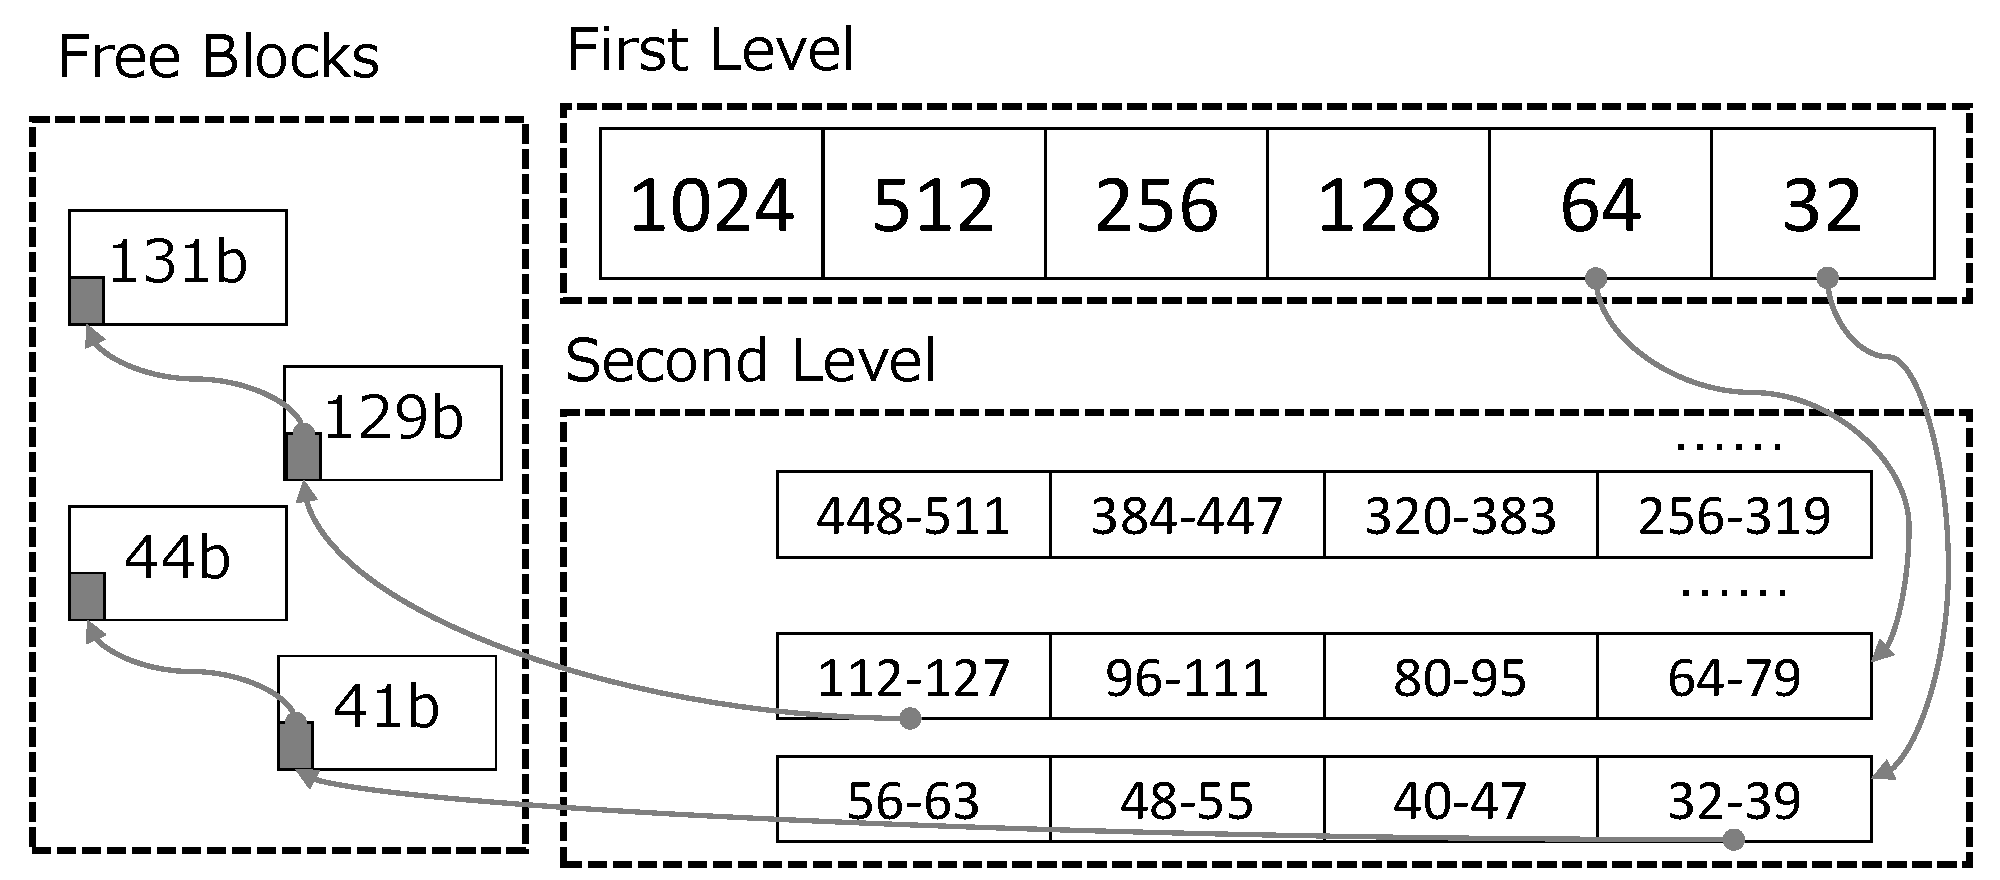
\includegraphics[width=8cm,clip]{figure/TLSF.pdf}
    \caption{TLSF algorithm}
    \label{fig:TLSF}
\end{figure}


\subsubsection{Component Design of TLSF+TECS}

In this subsection, we describe the component design of the TLSF memory allocator.
Note that we use TECS to componentize TLSF.
Further, the version of TLSF used is 2.4.6\footnote{http://www.gii.upv.es/tlsf/main/repo}.

\begin{figure}[t]
\centering
\begin{lstlisting}
signature sMalloc {
  int    initializeMemoryPool(void);
  void   *calloc([in]size_t nelem,[in]size_t size);
  void   *malloc([in]size_t size);
  void   *realloc([in]const void *ptr,[in]size_t size);
  void   free([in]const void *ptr);
};
\end{lstlisting}
\caption{Signature description of memory management}  
\label{src:TLSFSignature}
\end{figure}

In Fig.\ref{src:TLSFSignature}, we summarize the signature used by the allocator for dynamic memory management.
Particularly, this component defines the memory pool initialization function {\it initializeMemoryPool()}, memory allocation functions {\it calloc()}, {\it malloc()}, and {\it realloc()}, and the memory release function {\it free()}.

\begin{figure}[t]
\centering
\begin{lstlisting}
celltype tTLSFMalloc {
    [inline]entry  sMalloc  eMalloc;
    attr {
        size_t  memoryPoolSize;
    };
    var {
        [size_is(memoryPoolSize/8)]uint64_t *pool;
    };
};
\end{lstlisting}
\caption{Celltype description of TLSF memory allocator component}  
\label{src:TLSFCelltype}
\end{figure}

Next, Fig.\ref{src:TLSFCelltype} shows the celltype description for the TLSF memory allocator component.
Here, entry port {\it eMalloc} is connected to all components that perform memory management including $malloc()$ and $free()$.
Further, {\it [inline]} is a specifier to suggest to the TECS generator to implement as an inline function.
Memory pool size is defined as an attribute, and a pointer to a memory pool is defined as a variable.
Note that each component maintains its own heap area.
Therefore, even when calling memory management functions simultaneously from different threads, it is possible to operate without any memory contention.

\begin{figure}[t]
    \centering
    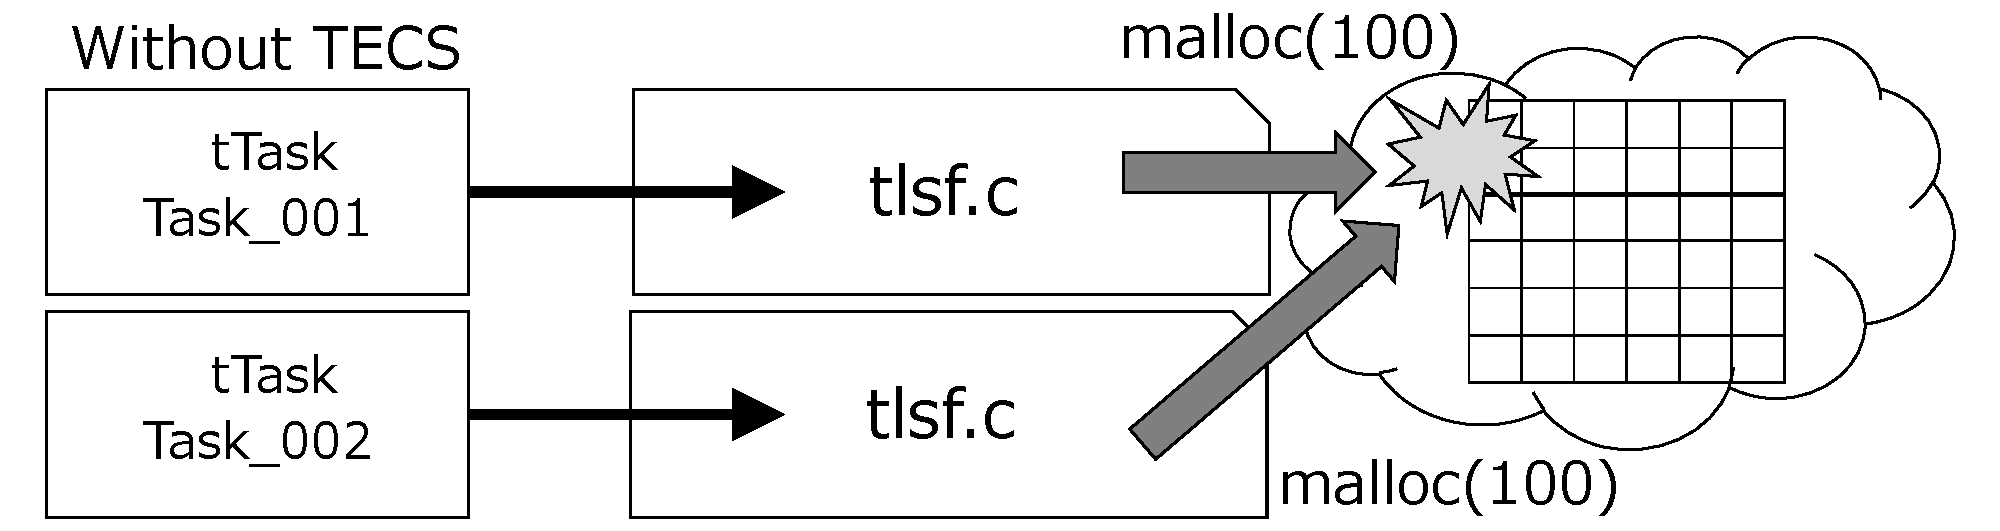
\includegraphics[width=8cm,clip]{figure/WithoutTECS.pdf}
    \caption{TLSF before componentization}
    \label{fig:WithoutTECS}
\end{figure}

\begin{figure}[t]
    \centering
    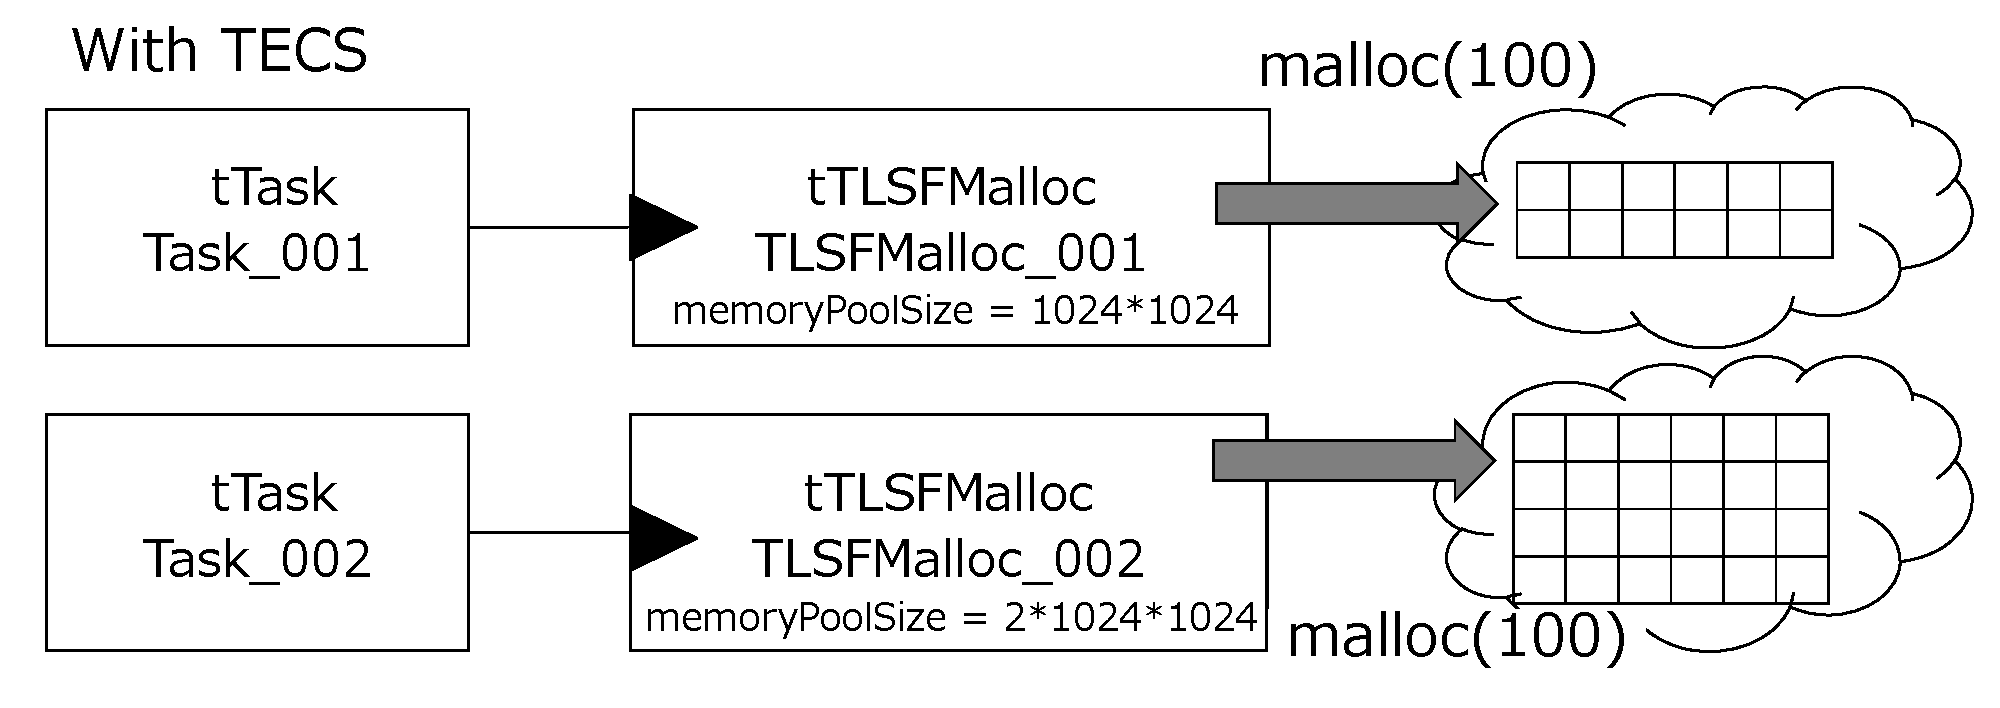
\includegraphics[width=8cm,clip]{figure/WithTECS.pdf}
    \caption{TLSF after componentization}
    \label{fig:WithTECS}
\end{figure}

As shown in Fig.\ref{fig:WithoutTECS}, since TLSF before componentization shares the heap area with multiple threads, if memory is allocated or released simultaneously via multiple threads, memory contention may occur in some cases, thus causing intermittent synchronization problems that can be extremely difficult to debug.
In this study, TLSF is componentized using TECS, as shown in Fig.\ref{fig:WithTECS}.
It is possible to operate in thread safe without exclusive control because each component independently holds a heap area and manages memory within it. 

\begin{figure}[t]
\centering
\begin{lstlisting}
cell tTask Task_001 {
    cMalloc = TLSFMalloc_001.eMalloc;
};
cell tTLSFMalloc TLSFMalloc_001 {
    memoryPoolSize = 1024*1024; /* 1MB */
};
cell tTask Task_002 {
    cMalloc = TLSFMalloc_002.eMalloc;
};
cell tTLSFMalloc TLSFMalloc_002 {
    memoryPoolSize = 2*1024*1024; /* 2MB */
};
\end{lstlisting}
\caption{Build description of TLSF memory allocator component}
\label{src:TLSFBuild}
\end{figure}


\begin{figure}[t]
\centering
\begin{lstlisting}
void*
mrb_TECS_allocf(mrb_state *mrb, void *p, 
                  size_t size, void *ud)
{
    CELLCB	*p_cellcb = (CELLCB *)ud;
    if (size == 0) {
        //tlsf_free(p);
        cMalloc_free(p);
        return NULL;
    }
    else if (p) {
        //return tlsf_realloc(p, size);
        return cMalloc_realloc(p, size);
    }
    else {
        //return tlsf_malloc(size);
        return cMalloc_malloc(size);
    }
}
\end{lstlisting}
\caption{Example of TLSF memory allocator component}  
\label{src:TLSFC}
\end{figure}

Next, Fig.\ref{src:TLSFBuild} shows the build description of the TLSF memory allocator component illustrated in Fig.\ref{fig:WithTECS}\footnote{Other call/entry ports, attributes, and valuables are actually described, but it is omitted here for simplicity.}.
Here, two sets of task components and TLSF components are combined.
Further, each memory pool size can be configured as a variable (lines 5 and 11 in Fig.\ref{src:TLSFBuild}).
Fig.\ref{src:TLSFC} presents the code that actually calls functions of the TLSF memory allocator component.
The use part shows a function in which the RiteVM allocates memory within the mruby on TECS framework\cite{par:mrubyonTECS}\cite{par:mrubyonTECS3}, which we introduced in Section \ref{sec:mrubyonTECS} above.
Line 8 calls the {\it free()} function of the TLSF memory allocator component.
{\it cMalloc\_} represents the name of the call port on line 2 in Fig.\ref{src:TLSFBuild}.
Similarly, lines 13 and 17 call the memory allocation function.
Particularly, the heap area for the {\it TLSFMalloc\_001} component is used if the code from \ref{src:TLSFC} is executed in {\it Task\_001}; conversely, if that code is executed in {\it Task\_002}, the heap area of the {\it TLSFMalloc\_002} component is used.
Using this approach, in component-based development using TECS, it is possible to operate with the same code without modifying the underlying C code, although the resulting cells differ.

\subsubsection*{Multiple RiteVM instances}

\begin{figure}[t]
    \centering
    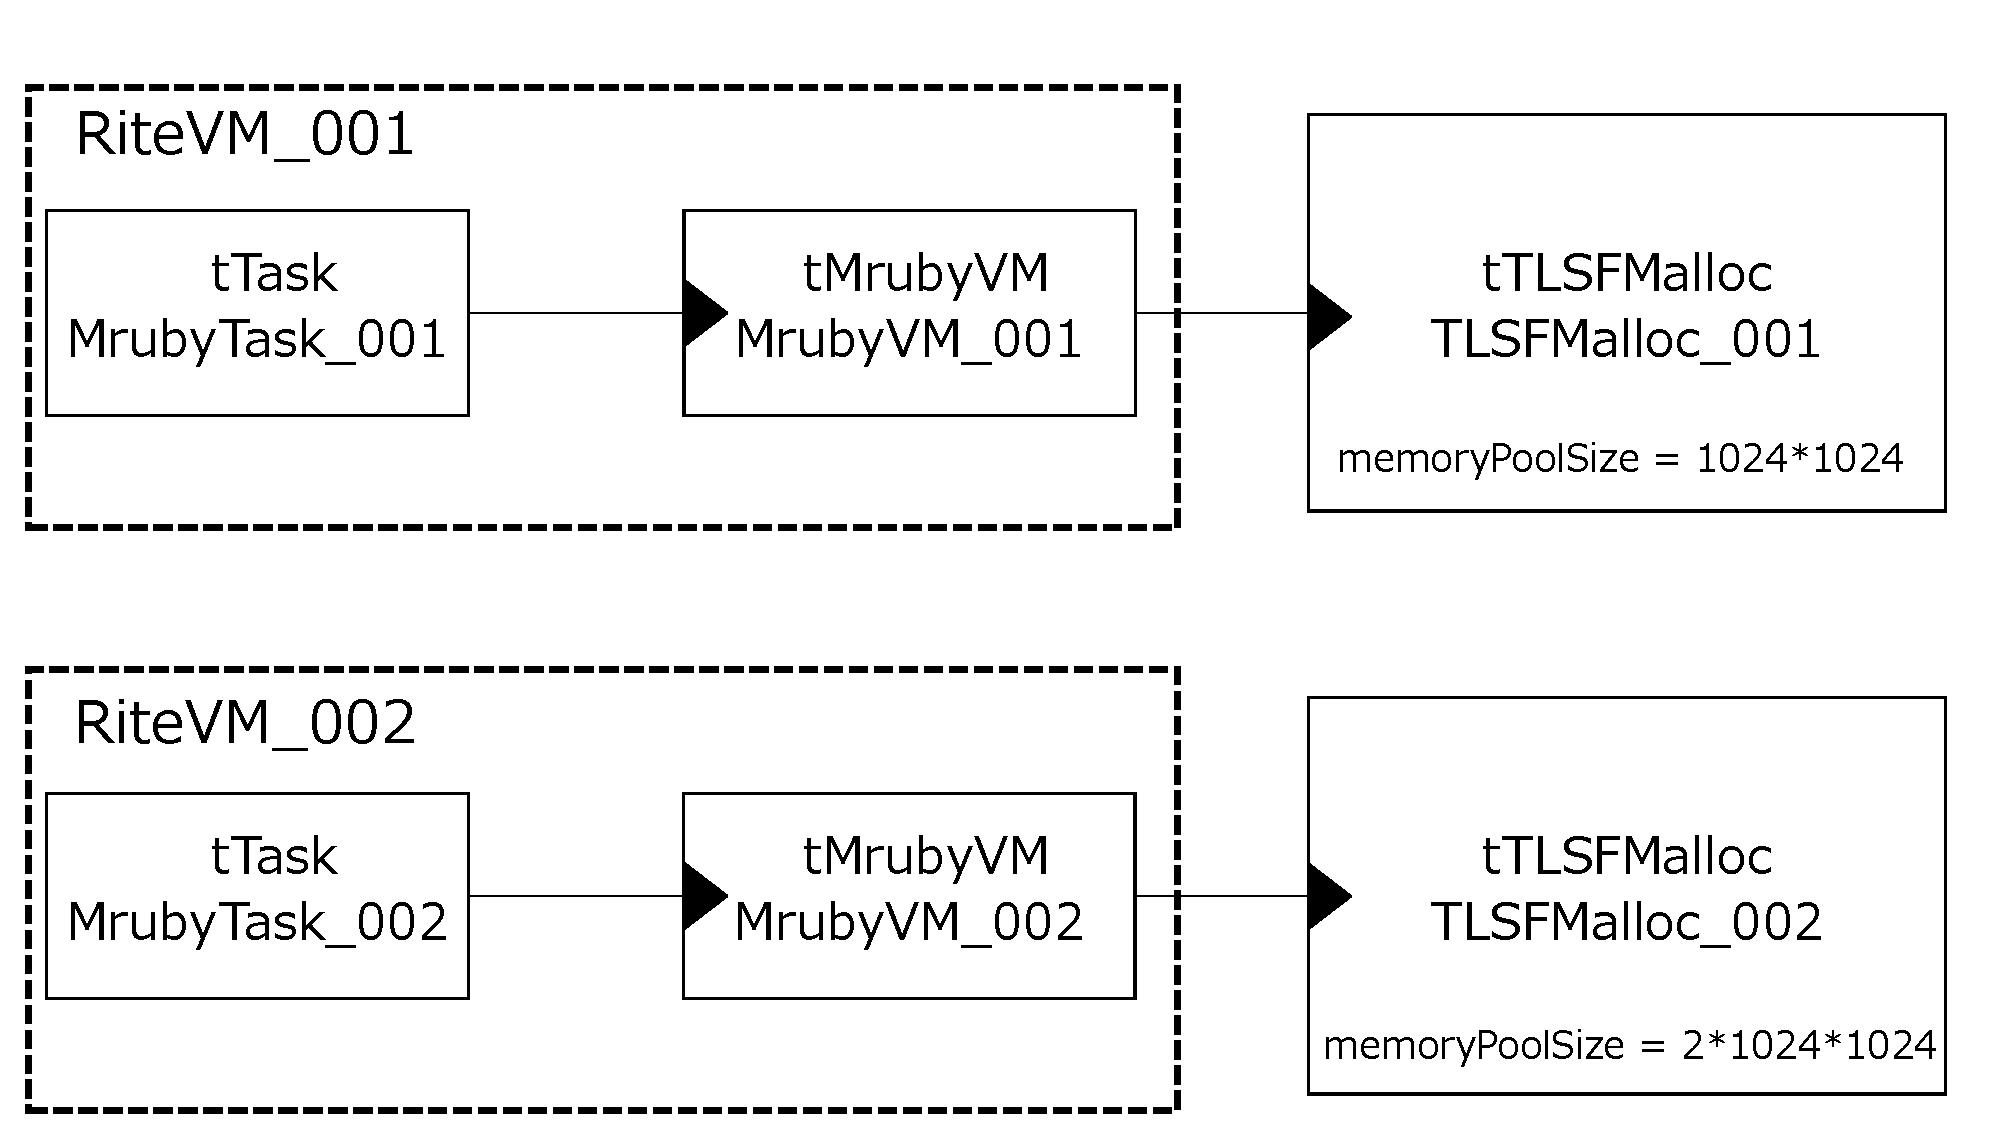
\includegraphics[width=8cm,clip]{figure/UseCase_mruby.pdf}
    \caption{Component description of RiteVM and TLSF+TECS}
    \label{fig:UseCase_mruby}
\end{figure}

The proposed framework uses the TLSF memory allocator for memory management within RiteVMs; however, since it is difficult to hundle multiple memory pools in the existing TLSF, if memory is allocated or deallocated from multiple threads, memory contention will likely occur.
Here, as a RiteVM allocates and deallocates memory at high frequencies, memory contention quickly occurs when multiple RiteVMs are instantiated.
Note that the TLSF components are connected to the RiteVMs to ensure that each component has its own heap area within each RiteVM, as illustrated in Fig.\ref{fig:UseCase_mruby}.
Since each TLSF component maintains its own memory pool, multiple RiteVMs can be executed without the possibility of any memory contention.
In Fig.\ref{fig:UseCase_mruby}, we observe that the first RiteVM has a heap area of 1 MB (i.e., 1024 $\times$ 1024 bytes) and the second RiteVM has a heap area of 2 MB (i.e., 2 $\times$ 1024 $\times$ 1024 bytes).
As illustrated in Fig.\ref{fig:UseCase_mruby}, it is easy to configure different-sized heap areas for each RiteVM.
Further, each RiteVM performs incremental garbage collection (GC), and a RiteVM that has started GC does not disturb the execution of other RiteVMs in its GC execution.
    
\subsubsection*{Memory management for sending and receiving data}

\begin{figure}[t]
    \centering
    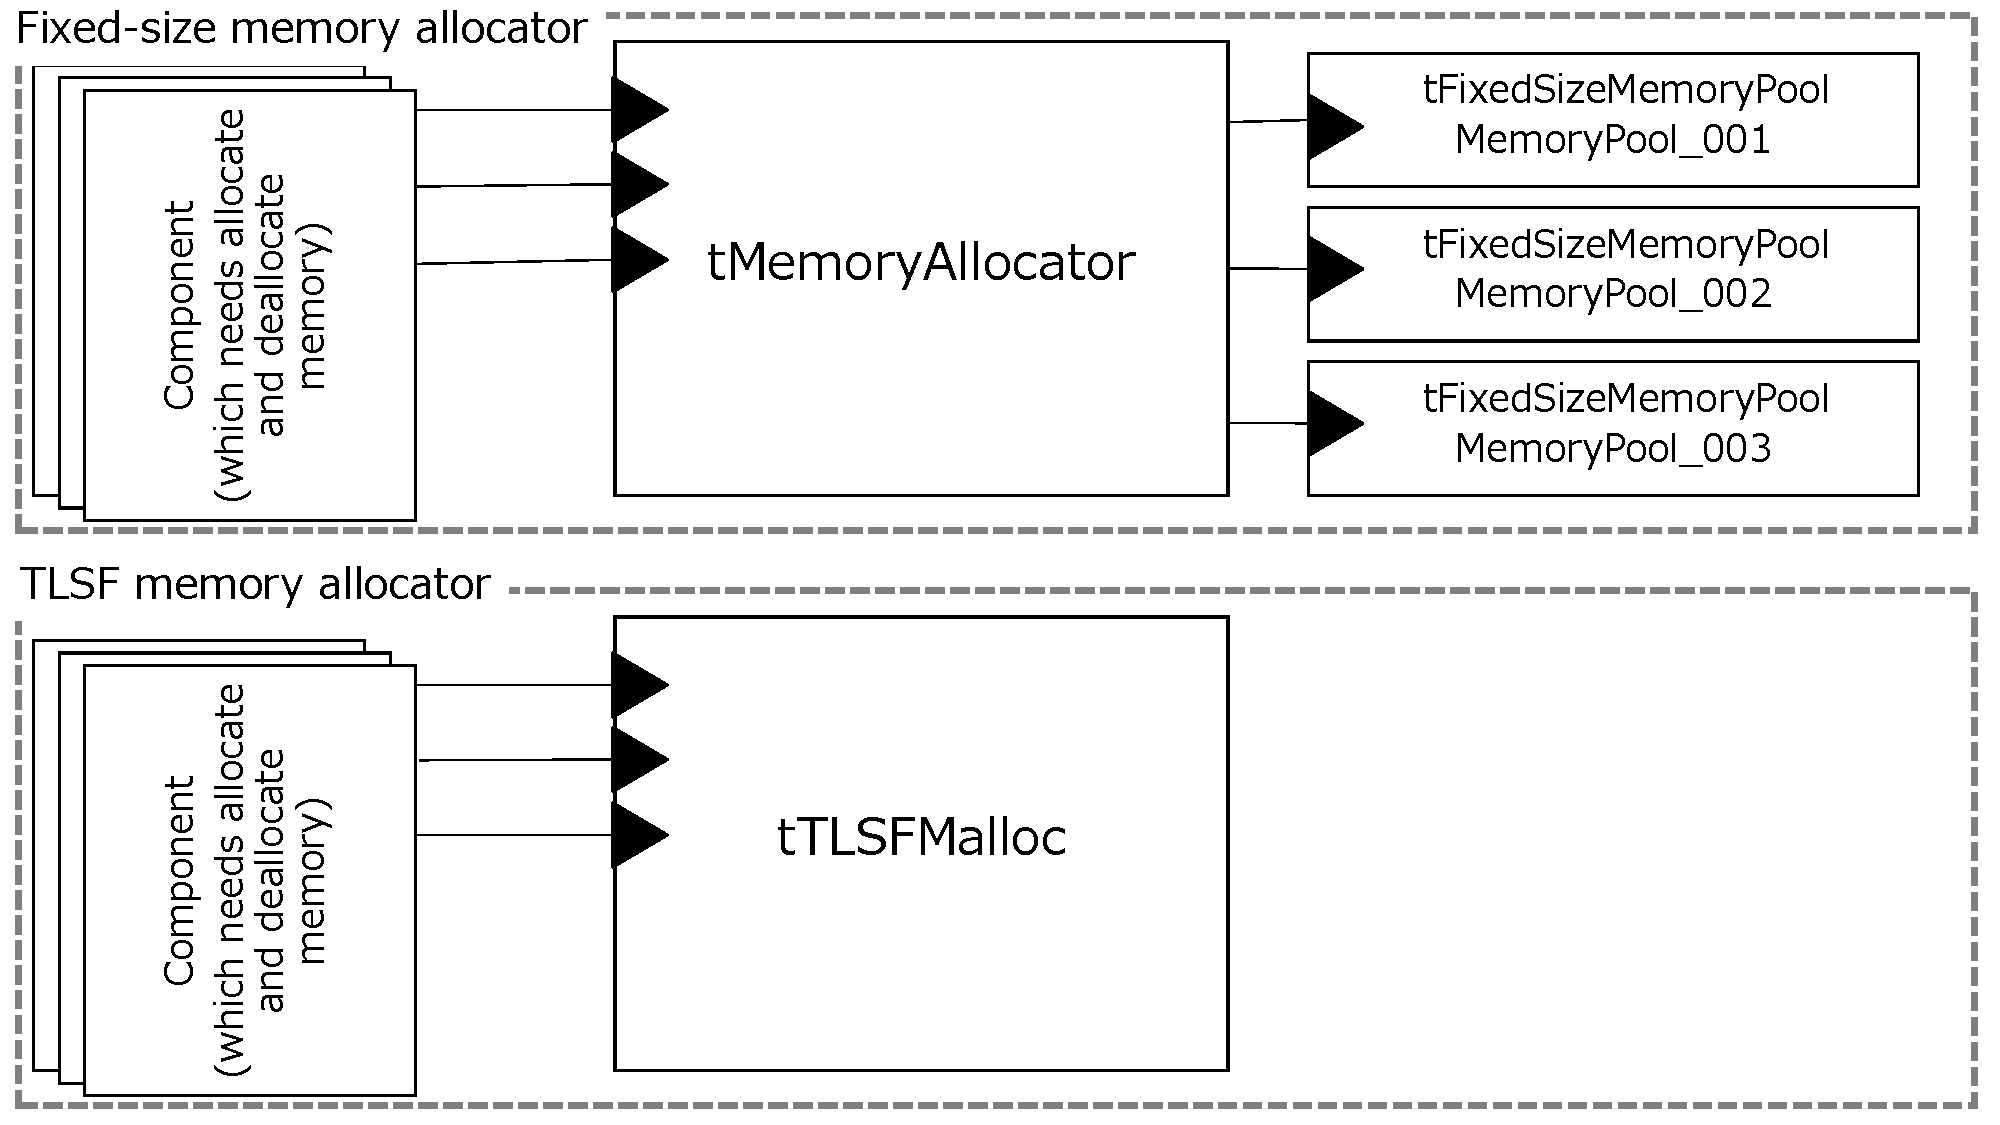
\includegraphics[width=8cm,clip]{figure/UseCase_TINET.pdf}
    \caption{Fixed-size and TLSF memory allocator components}
    \label{fig:UseCase_TINET}
\end{figure}

In the TCP/IP protocol stack, memory allocation and subsequent deallocation are repeated in each layer, including the TCP, IP, Ethernet, and other layers.
Therefore, the role of the memory allocator is critical.
The TINET+TECS framework combines all components that manage memory within the allocator.
The TLSF memory allocator can execute at the same speed as that of the fixed-size memory allocator that TOPPERS/ASP3 supports as standard; further, the TLSF memory allocator can improve memory efficiency.
As illustrated in Fig.\ref{fig:UseCase_TINET}, the fixed-size memory allocator prepares memory pools of different sizes and selects a memory pool whenever it is necessary.
Conversely, TLSF+TECS efficiently manages memory without the need to select a memory pool.
Finally, TLSF+TECS can be easily extended to TINET+TECS since TINET+TECS is a component-based system.

\subsection{Use case}
\label{sec:UseCase}

In the proposed framework, applications can call TINET functions, such as specific TCP- and UDP-related functions, from mruby programs because the mruby-TECS bridge automatically generates the code to link mruby and C.
Fig.\ref{src:mruby} shows an example of mruby program that transmits the value acquired from the sensor to another device or a server.
In general, mruby makes it easier to develop applications than using C with the existing TINET.

For a simple application, typically only a few functions are used, with numerous unused functions.
As an example, the application code shown in Fig.\ref{src:mruby} only uses a function to send data via TCP.
The proposed framework incorporates TINET+TECS and can easily customize the TCP/IP protocol stack by removing functions, such as UDP functions, functions that support only IPv4, or TCP receiving functions.
As such, the proposed framework can be applied to embedded systems with strict memory constraints by removing many unused functions.


\begin{figure}[t]
\centering
\begin{lstlisting}[language=Ruby]
begin
    io = AnalogIO.new(A0, INPUT)
    cep = TCP.new()	
    cep.accept
    loop do		
        val = io.read  
        cep.send val.to_s + "\n"		
        RTOS.delay(1000)			
    end
rescue => e	
    puts "[ERROR]" + e
end
\end{lstlisting}
\caption{An example of mruby application}
\label{src:mruby}
\end{figure}

%4
\section{Evaluation}
\label{sec:Evaluation}

This section describes the experimental evaluation used to demonstrate the effectiveness of the proposed framework.
GR-PEACH was employed as the evaluation board.
Detailed specifications of the board are shown in Table \ref{tab:EvaluationBoardEnvironment}.
We also employ TINET 1.5.4 and the compiler arm-none-eabi-gcc 5.2
To pretest the system, we connected the board to a host PC via a LAN cable and evaluated the data sending and receiving.

\begin{table}[t]
    \centering
    \caption{Evaluation Board Environment}
    \begin{tabular}{l|l}
        \hline\hline
        Board           &   GR-PEACH                \\
        CPU             &   Cortex-A9 RZ/A1H 400MHz \\
        Flash ROM       &   8 MB                    \\
        RAM             &   10 MB                   \\
        LAN Controller  &   LAN8710A                \\
        \hline
    \end{tabular}
    \label{tab:EvaluationBoardEnvironment}
\end{table}

\subsection{Improved configurability}

As shown in Table \ref{tab:EvaluationOfConfigurability}, the code lines for modification were measured to demonstrate the improved configurability.
This demonstrated the ability to change the composition of the protocol stack with a small workload, confirming that the proposed framework improves the configurability.

\begin{table}[t]
    \centering
    \caption{Modified code lines of CDL}
    \begin{tabular}{c|r|r|r}
        \hline\hline
                         &   Size       &   Size (-- Default) & CDL  \\ \hline
        Default          &   325.23 KB  &              0 KB   &  0 lines   \\
        I                &   305.40 KB  &       -- 19.83 KB   & 18 lines   \\
        I + I\hspace{-.1em}I &   304.12 KB  &   -- 21.10 KB   & 27 lines   \\
        I + I\hspace{-.1em}I + I\hspace{-.1em}I\hspace{-.1em}I & 303.45 KB & -- 21.77 KB  & 32 lines \\
        \hline
        \multicolumn{4}{l}{I: Remove TCP}\\
        \multicolumn{4}{l}{I\hspace{-.1em}I: Remove ICMP}\\
        \multicolumn{4}{l}{I\hspace{-.1em}I\hspace{-.1em}I: Change network buffer (Remove memory pools)}
    \end{tabular}
    \label{tab:EvaluationOfConfigurability}
\end{table}

\subsection{Performance of TINET+TECS}

To demonstrate the low overhead of TINET+TECS, we compared its execution time and memory consumption with that of TINET.
The results with TCP are shown in Fig.\ref{fig:EvaluationOfExecutionTime}.
The {\it tcp\_snd\_dat} and {\it tcp\_rcv\_dat} APIs were used in the evaluation to, respectively, send and receive TCP data.
For {\it tcp\_snd\_dat}, we measured the executing time starting from the API call through the application until the return of the processing result.
In TINET+TECS, this process is performed in the order tApplication, tTCPCEP, tTCPOutputTaskBody, tIPv4Output, tEthernetOutput, tArp, tEthernetOutputTaskBody, and tIfMbed, as shown in Fig.\ref{fig:ComponentProtocolStack}.
For {\it tcp\_rcv\_dat}, we measured the execution time from the data receipt in the LAN driver until data acquisition in the application.
In TINET+TECS, the process is performed in the order tIfMbed, tEthernetInputTaskBody, tIPv4Input, tTCPInput, tTCPCEP, and tApplication, as shown in Fig.\ref{fig:ComponentProtocolStack}.
The execution time of TINET+TECS is close to that of TINET, with an overhead of about 3 us.
Conversely, we evaluated the execution times with UDP as shown in Fig.\ref{fig:EvaluationOfExecutionTimeUDP}.
TINET+TECS can run at the same speed as TINET; therefore, the overheads of TINET+TECS are low.
As the use of the {\it send/receive} specifier enables accessing of the buffer address without data copying, the componentization overhead does not affect the execution time.

\begin{figure}[t]
    \centering
    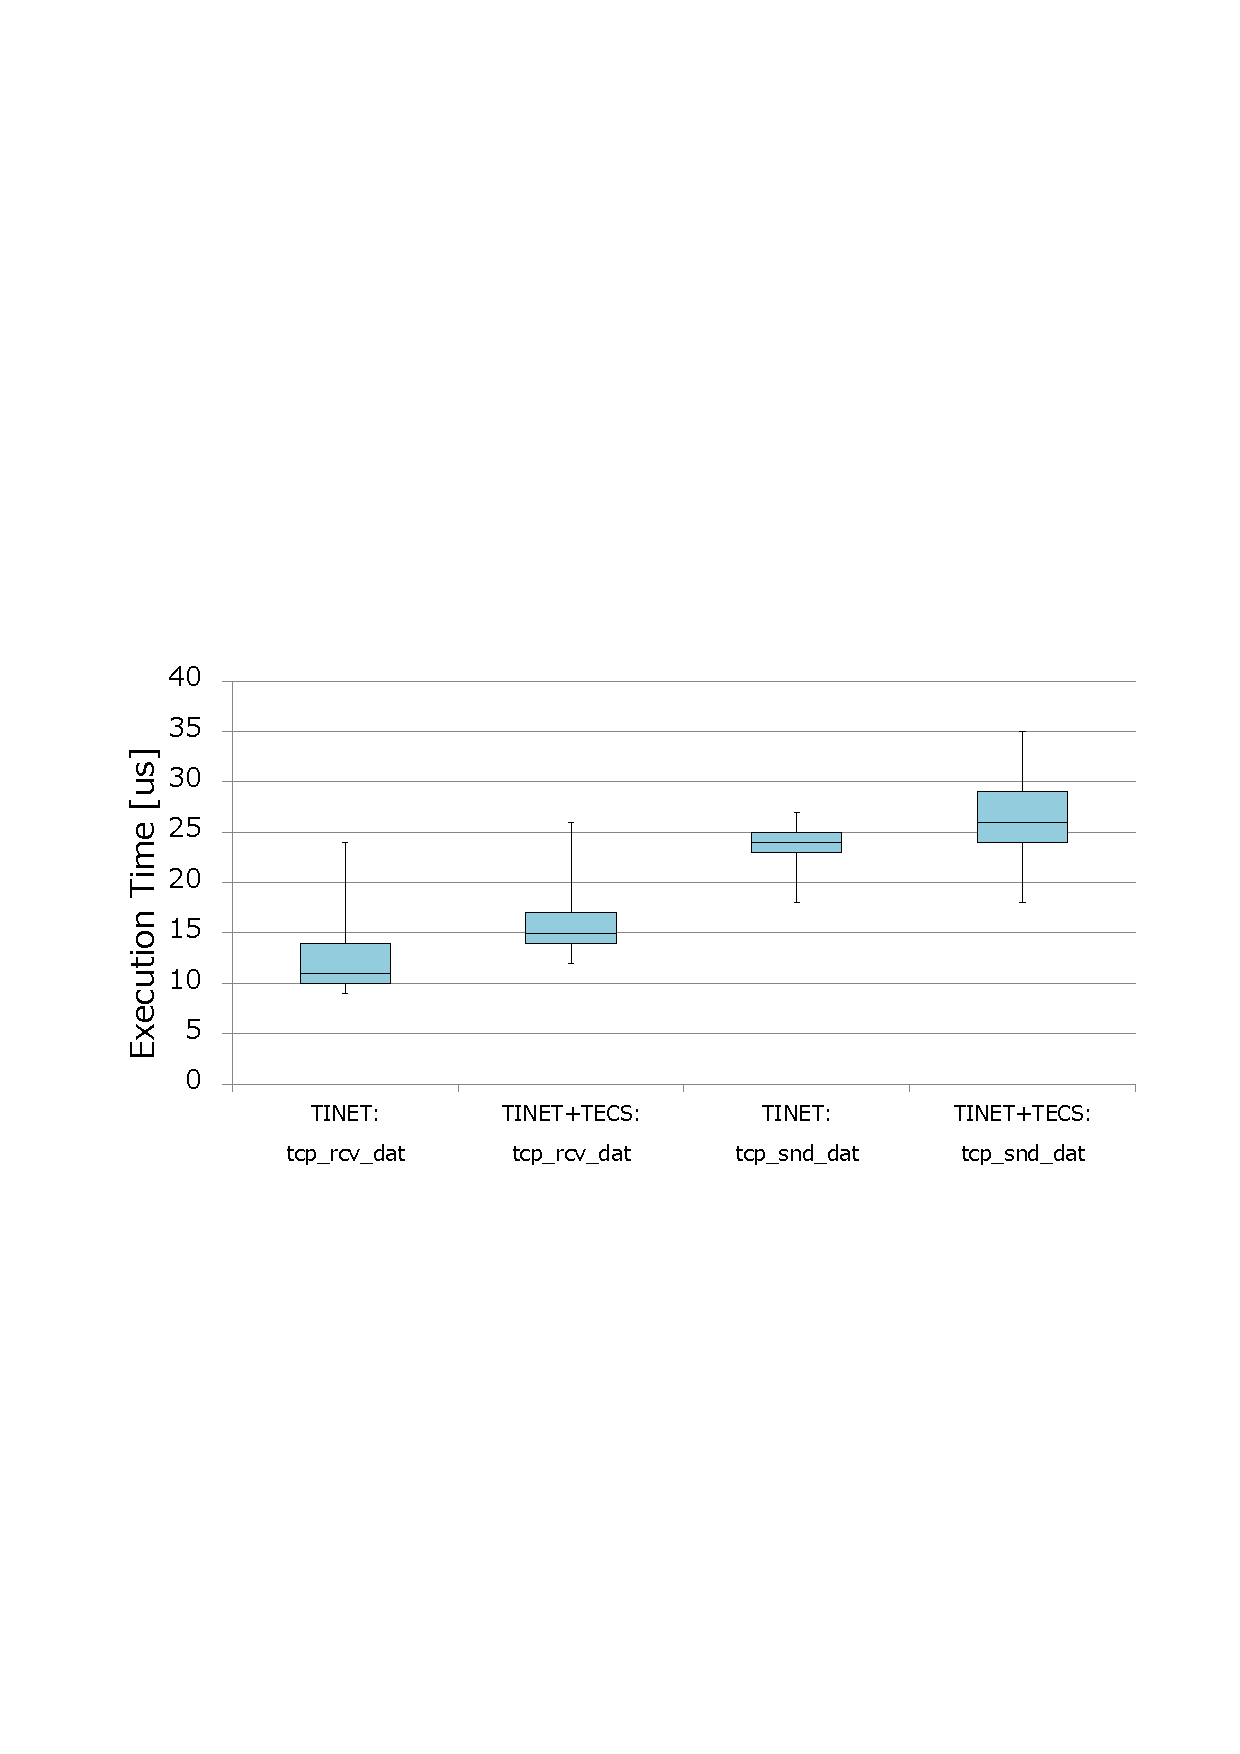
\includegraphics[width=8cm,clip]{figure/EvaluationOfExecutionTime.pdf}
    \caption{Execution times of TINET and TINET+TECS with TCP}
    \label{fig:EvaluationOfExecutionTime}
\end{figure}

\begin{figure}[t]
    \centering
    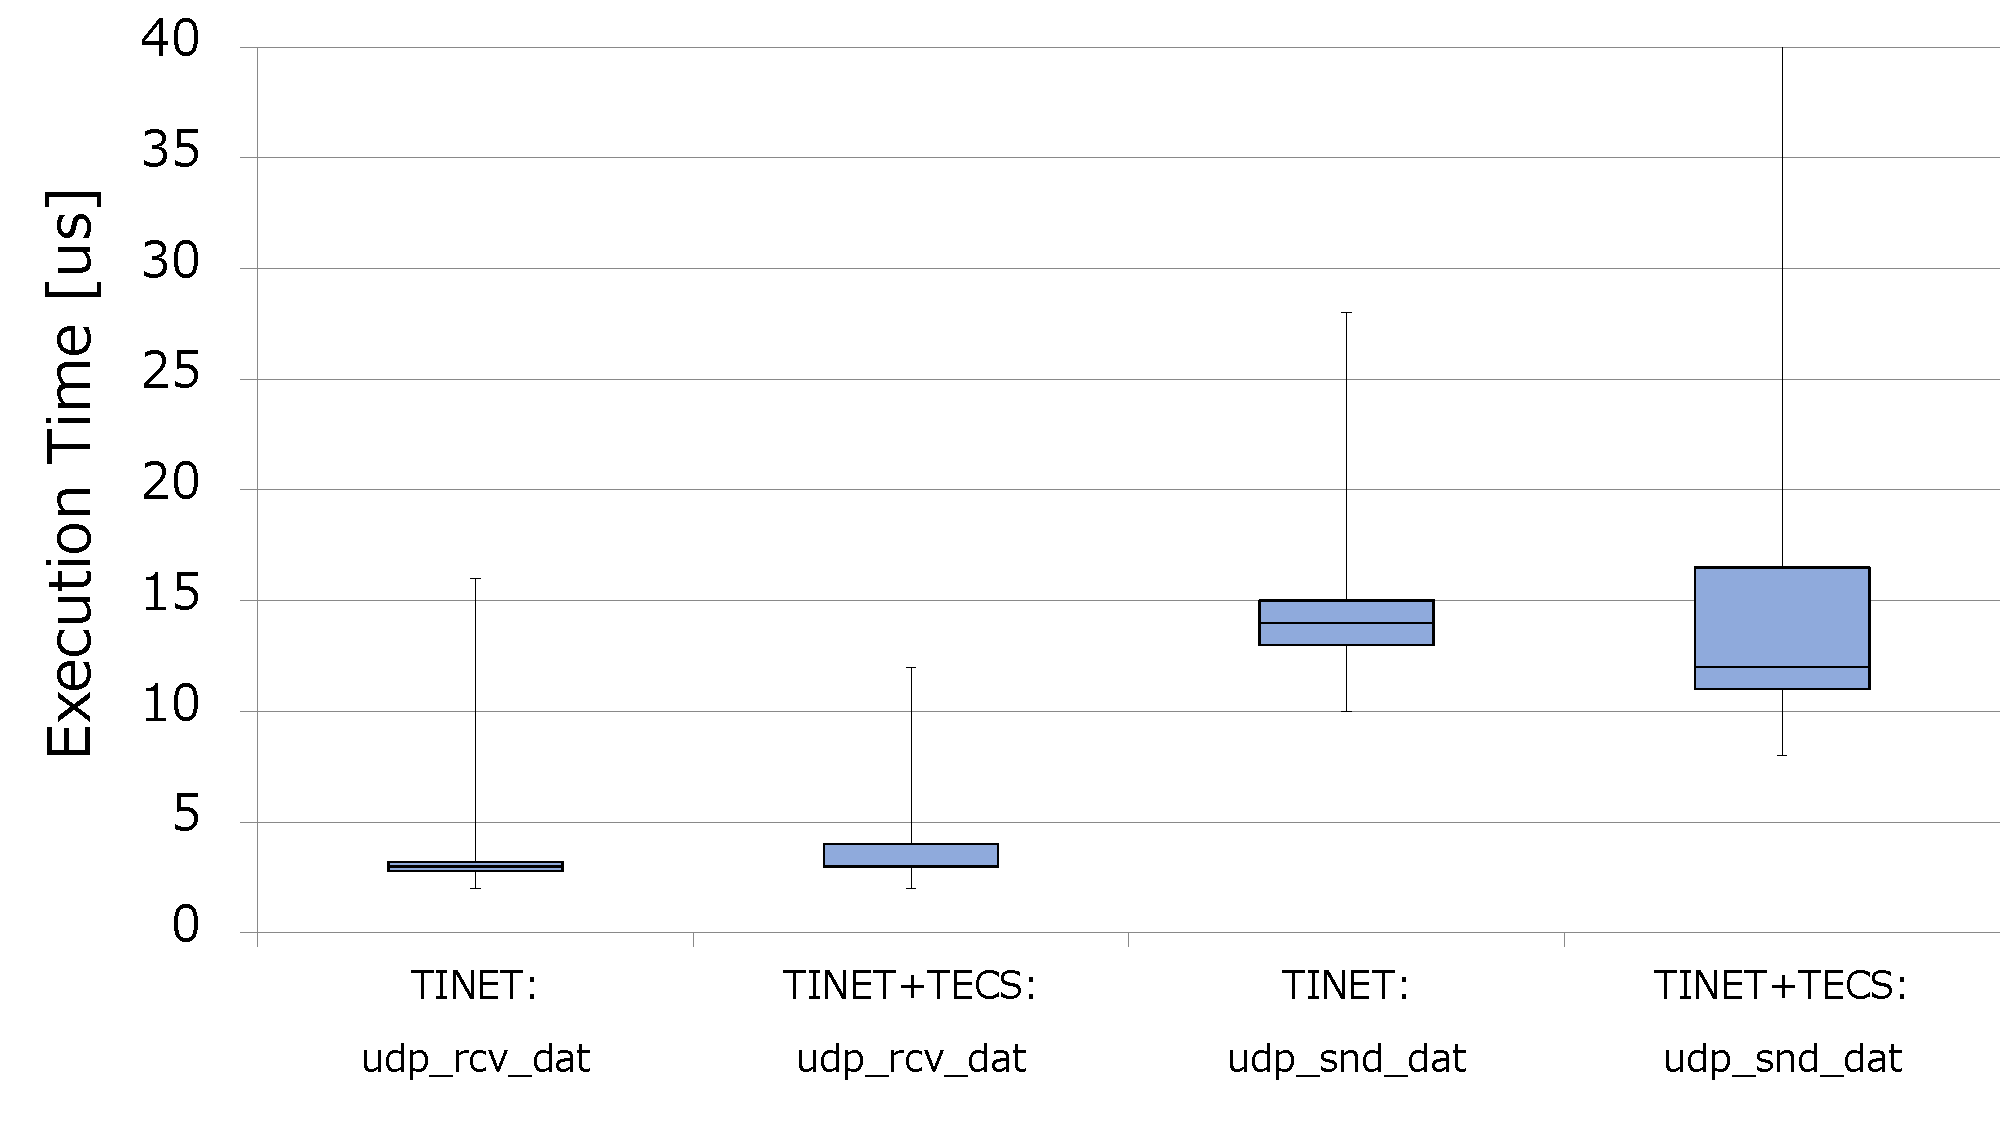
\includegraphics[width=8cm,clip]{figure/EvaluationOfExecutionTimeUDP.pdf}
    \caption{Execution times of TINET and TINET+TECS with UDP}
    \label{fig:EvaluationOfExecutionTimeUDP}
\end{figure}

The memory consumptions of TINET and TINET+TECS are compared in Table \ref{tab:EvaluationOfMemoryConsumption}.
The memory consumption of TINET+TECS is about 1\% higher than that of TINET, as the data and processes such as initialization of cells, descriptors, function tables, and skeleton functions needed to manage TECS components increase memory consumption.

\begin{table}[t]
    \centering
    \caption{Memory consumption of TINET and TINET+TECS}
    {\tabcolsep = 1mm
    \begin{tabular}{c|r|r|r|r}
        \hline\hline
                               &   text       &  data    &   bss      &  total     \\ \hline
        TINET                  &   183.94 KB  &  5.37 KB &  132.03 KB &  322.34 KB \\
        TINET+TECS (TCP)       &   169.48 KB  &  5.37 KB &  149.01 KB &  323.96 KB \\
        TINET+TECS (UDP)       &   169.26 KB  &  5.37 KB &  149.04 KB &  323.77 KB \\
        TINET+TECS (TCP+UDP)   &   170.73 KB  &  5.37 KB &  149.13 KB &  325.23 KB \\
        \hline
        \multicolumn{5}{r}{Including the application and kernel objects}
    \end{tabular}
    }
    \label{tab:EvaluationOfMemoryConsumption}
\end{table}

\subsection{Dynamic connection}

\begin{figure}[t]
    \centering
    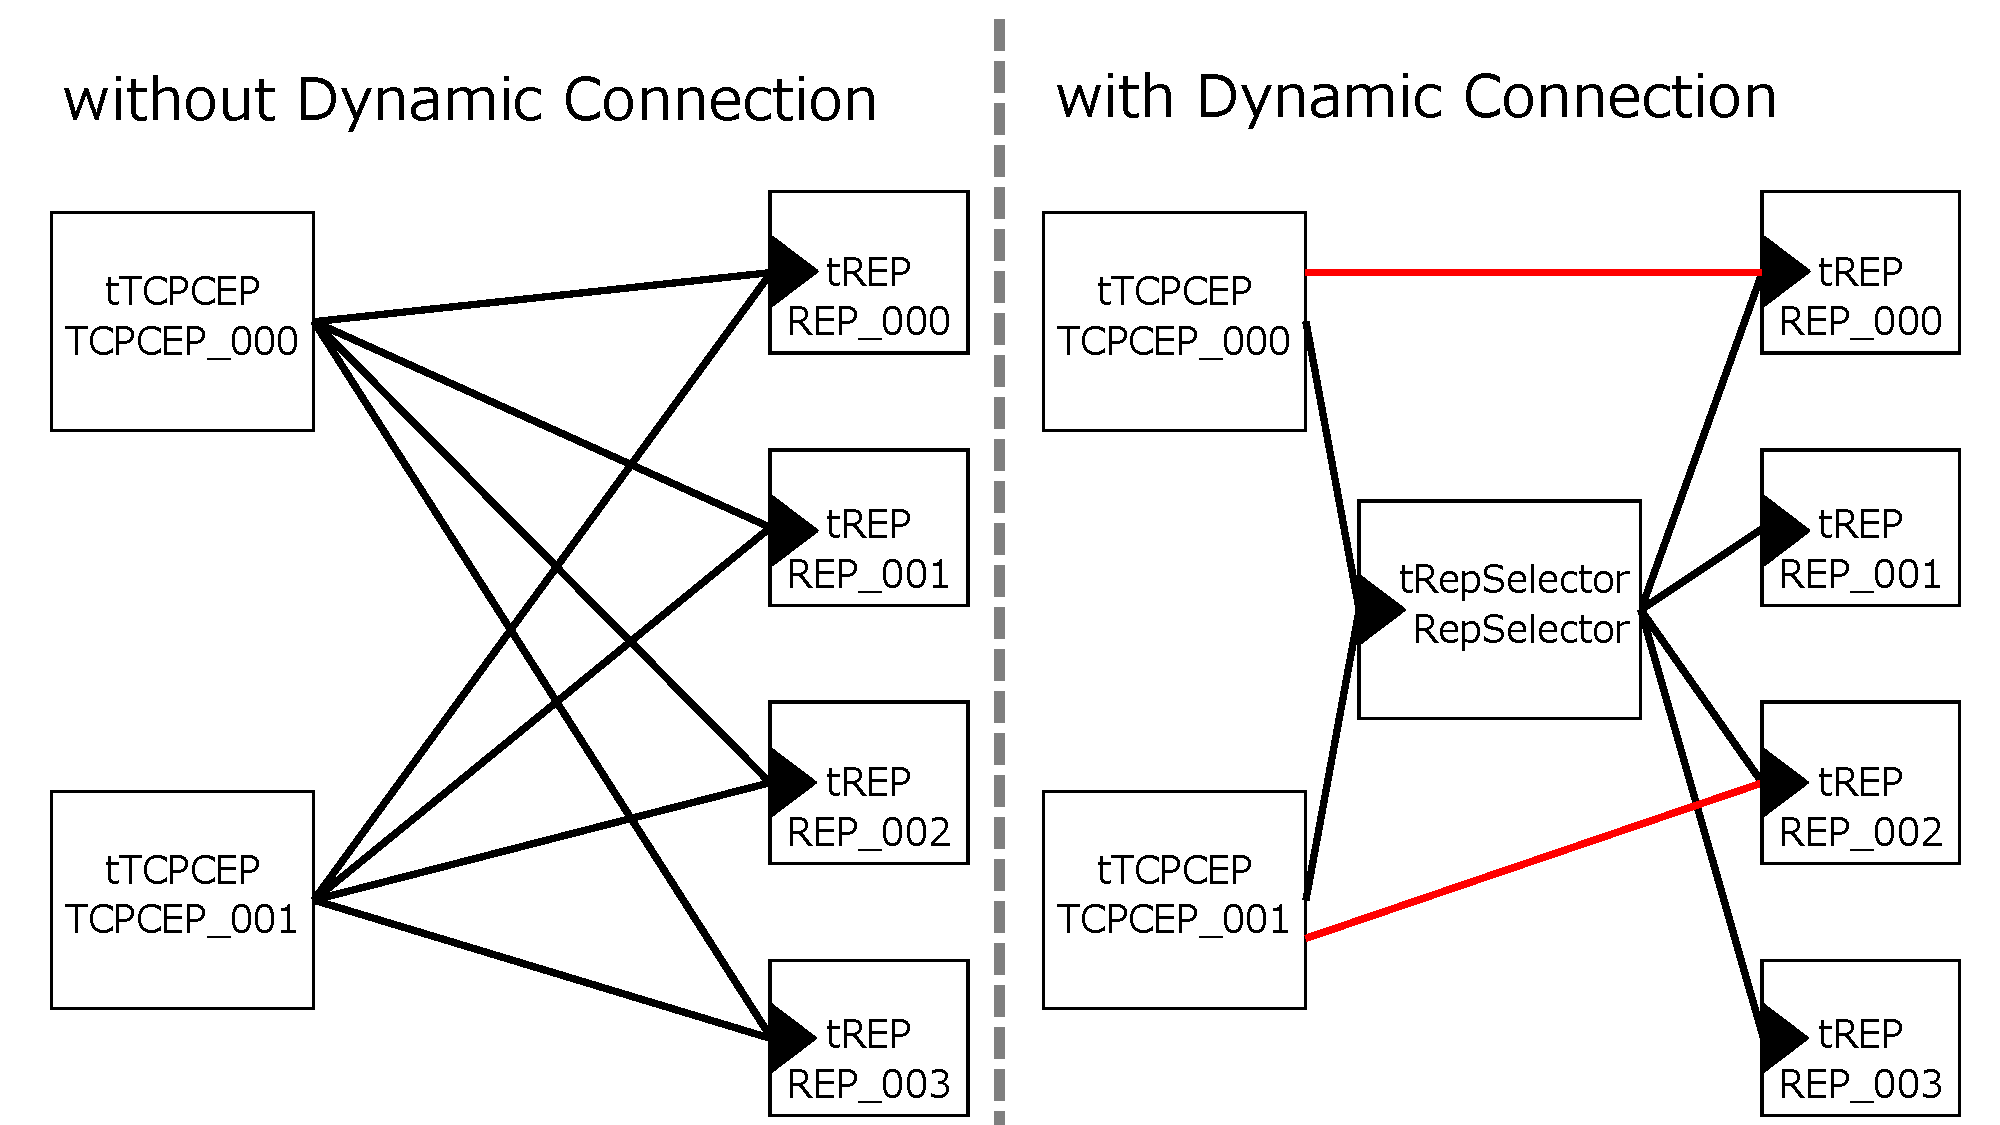
\includegraphics[width=8cm,clip]{figure/ComparisonOfDynamicConnection.pdf}
    \caption{Component diagrams for without/with dynamic connection}
    \label{fig:ComparisonOfDynamicConnection}
\end{figure}

Memory consumption without and with TECS dynamic connection was then evaluated.
As shown in the left of Fig.\ref{fig:ComparisonOfDynamicConnection}, each CEP component should be statically connected to all REP components if the dynamic connection is not used.
As the number of REPs increases, additional call ports of CEP are required, in turn increasing the consumption of memory. 
The dynamic connection reduces memory consumption because only one CEP-to-REP call port is required per CEP, as illustrated with red lines in the right paneof Fig.\ref{fig:ComparisonOfDynamicConnection}.
Even if the number of REPs increases, additional call ports can be joined through the selector, instead of the CEPs.

Memory consumption of without and with dynamic connection is shown in TABLE \ref{fig:EvaluationOfDynamicConnection}.
The dynamic connection case consumes the more RAM memory because, as mentioned in Section \ref{sec:DynamicConnection}, call ports with {\it [dynamic]} are not optimized and allocated in RAM areas.
However, the overall memory consumption is lower under the proposed framework.

% \begin{figure}[t]
%     \centering
%     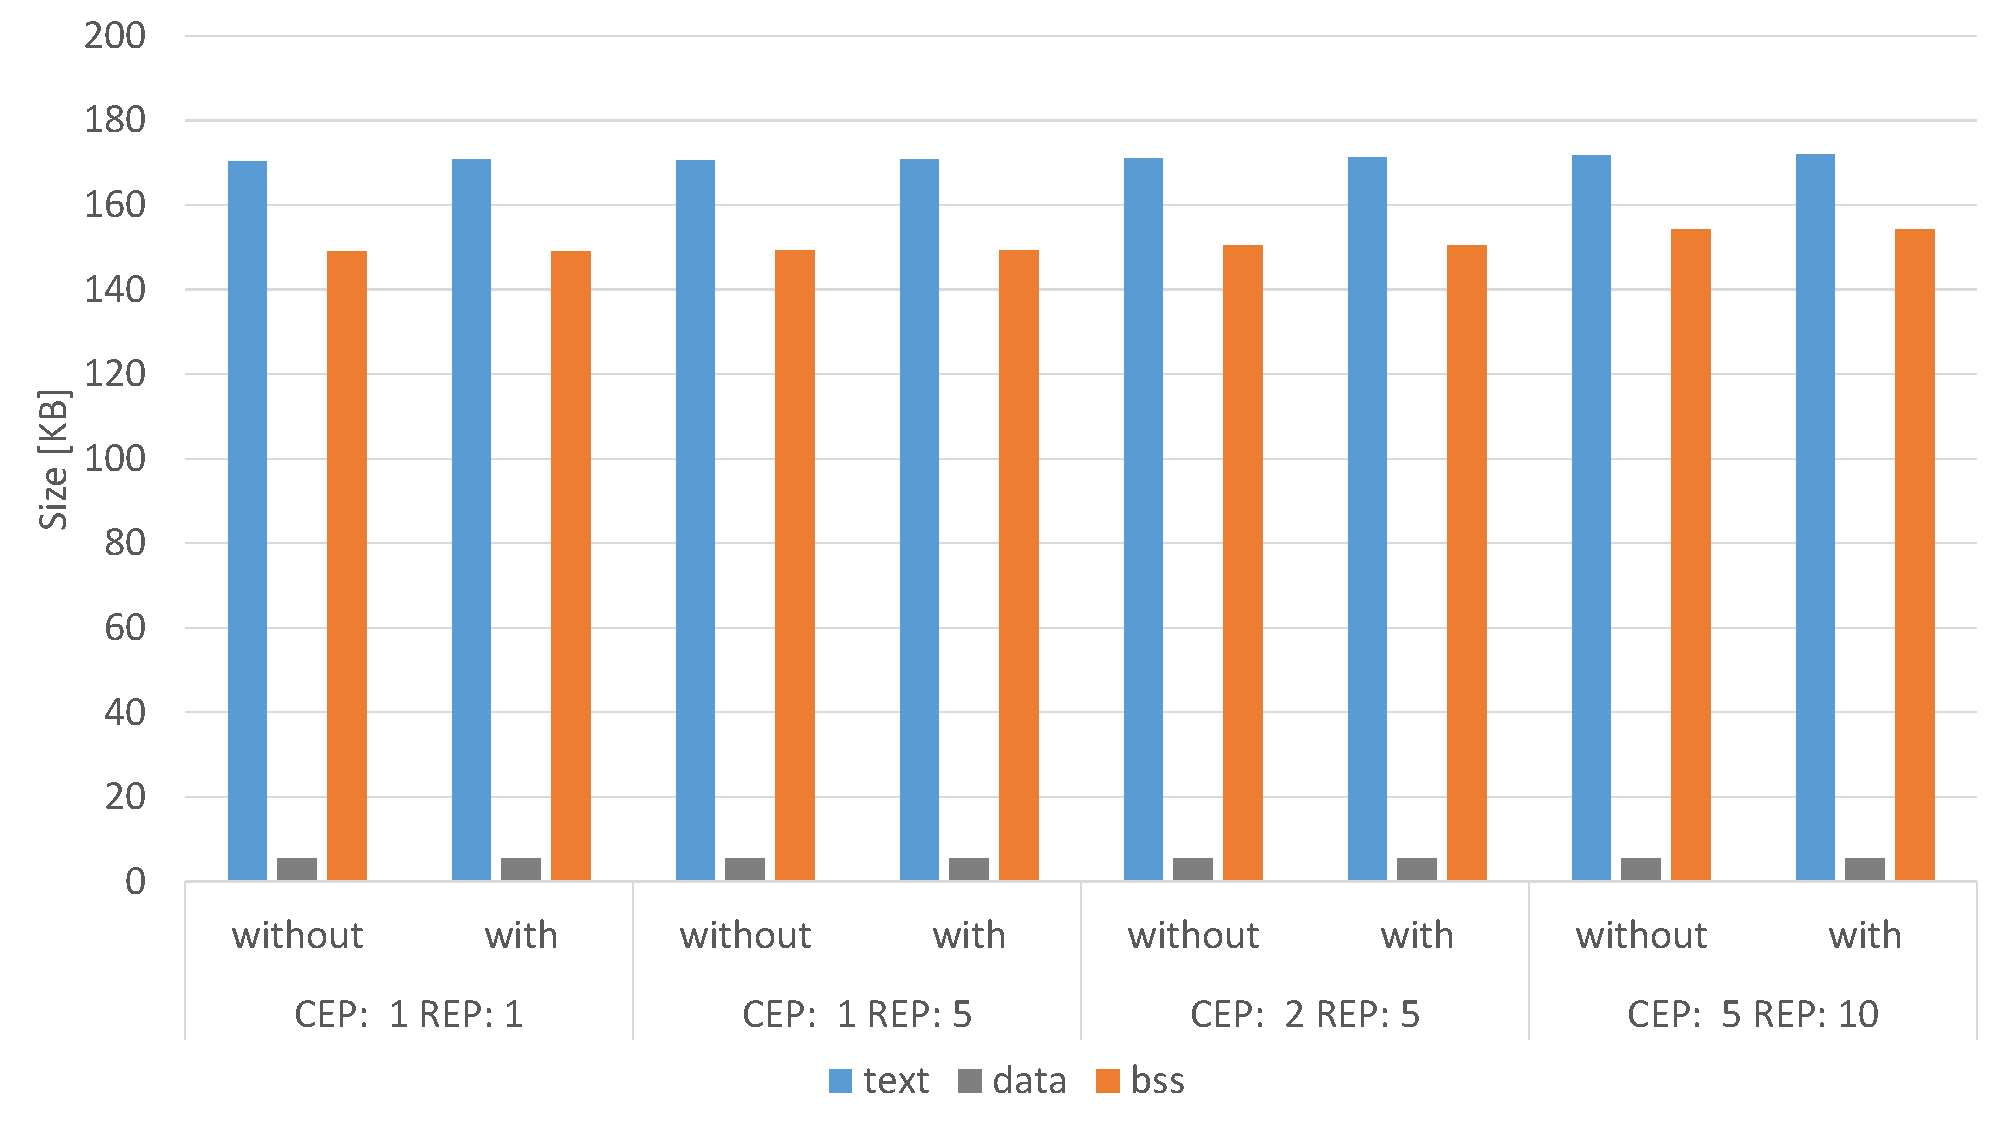
\includegraphics[width=8.0cm,clip]{figure/EvaluationOfDynamicConnection.pdf}
%     \caption{Memory consumption in two cases (with/without dynamic connection)}
%     \label{fig:EvaluationOfDynamicConnection}
% \end{figure}
\begin{table}[t]
    \centering
    \caption{Memory consumption in two cases\\(with/without dynamic connection)}
    {\tabcolsep = 1mm
    \begin{tabular}{c|r|r|r|r}
        \hline\hline
                &  CEP:1 REP:1 & CEP:1 REP:5 & CEP:2 REP:5 & CEP:5 REP:10 \\ \hline
        without &  324.98 KB   & 325.34 KB   & 326.39 KB   & 331.68 KB   \\
        with    &  325.23 KB   & 325.32 KB   & 327.24 KB   & 330.48 KB   \\
        \hline
    \end{tabular}
    }
    \label{fig:EvaluationOfDynamicConnection}
\end{table}

\begin{table}[t]
    \centering
    \caption{CDL code lines of without/with dynamic connection}
    \begin{tabular}{l|r|r|r}
        \hline\hline
                     &  without  &  with  &  Diff  \\ \hline
        CEP:1 REP:1  &  344 lines     &  347 lines  &  -3 lines   \\
        CEP:1 REP:5  &  369 lines     &  367 lines  &   2 lines   \\
        CEP:2 REP:5  &  387 lines     &  382 lines  &   5 lines   \\
        CEP:5 REP:10 &  485 lines     &  445 lines  &  40 lines   \\
        \hline
    \end{tabular}
    \label{tab:EvaluationOfConfigurabilityByDynamicConnection}
\end{table}

\begin{figure}[t]
 \centering
 \begin{lstlisting}
/* without Dynamic Connection */
cell tTCPCEP TCPCEP_000 {
    cREP[0] = REP_000.eREP;
    ..
    cREP[n] = REP_00n.eREP;
};
cell tTCPCEP TCPCEP_001 {
    cREP[0] = REP_000.eREP;
    ..
    cREP[n] = REP_00n.eREP;
};
..
cell tTCPCEP TCPCEP_00n {
    cREP[0] = REP_000.eREP;
    ..
    cREP[n] = REP_00n.eREP;
};
 \end{lstlisting}
 \centering
 \begin{lstlisting}
/* with Dynamic Connection */
cell tRepSelector RepSelector {
    cREP[0] = REP_000.eREP;
    ..
    cREP[n] = REP_00n.eREP;
};
cell tTCPCEP TCPCEP_000 {
    cRepSelector = RepSelector.eRepSelector;
};
cell tTCPCEP TCPCEP_001 {
    cRepSelector = RepSelector.eRepSelector;
};
..
cell tTCPCEP TCPCEP_00n {
    cRepSelector = RepSelector.eRepSelector;
};
 \end{lstlisting}
 \caption{Two CDL codes (without/with dynamic connection)}
 \label{src:ComparisonOfCDL}
\end{figure}

The code lines in CDL of without and with the dynamic connection is shown in TABLE \ref{tab:EvaluationOfConfigurabilityByDynamicConnection} to demonstrate improved configurability.
As the number of CEPs and REPs increases, the amount of CDL code lines to be added increases.
In the left of Fig.\ref{fig:ComparisonOfDynamicConnection}, each CEP connects all REPs as shown in the upper of Fig.\ref{src:ComparisonOfCDL}. 
In the right of Fig.\ref{fig:ComparisonOfDynamicConnection}, a CEP dynamically connects an REP, and only the selector connects all REPs as shown in the lower of Fig.\ref{src:ComparisonOfCDL}. 
It is effective for software that uses many ports because the difference spreads as the number of CEPs and REPs increases.



\begin{figure}[t]
    \centering
    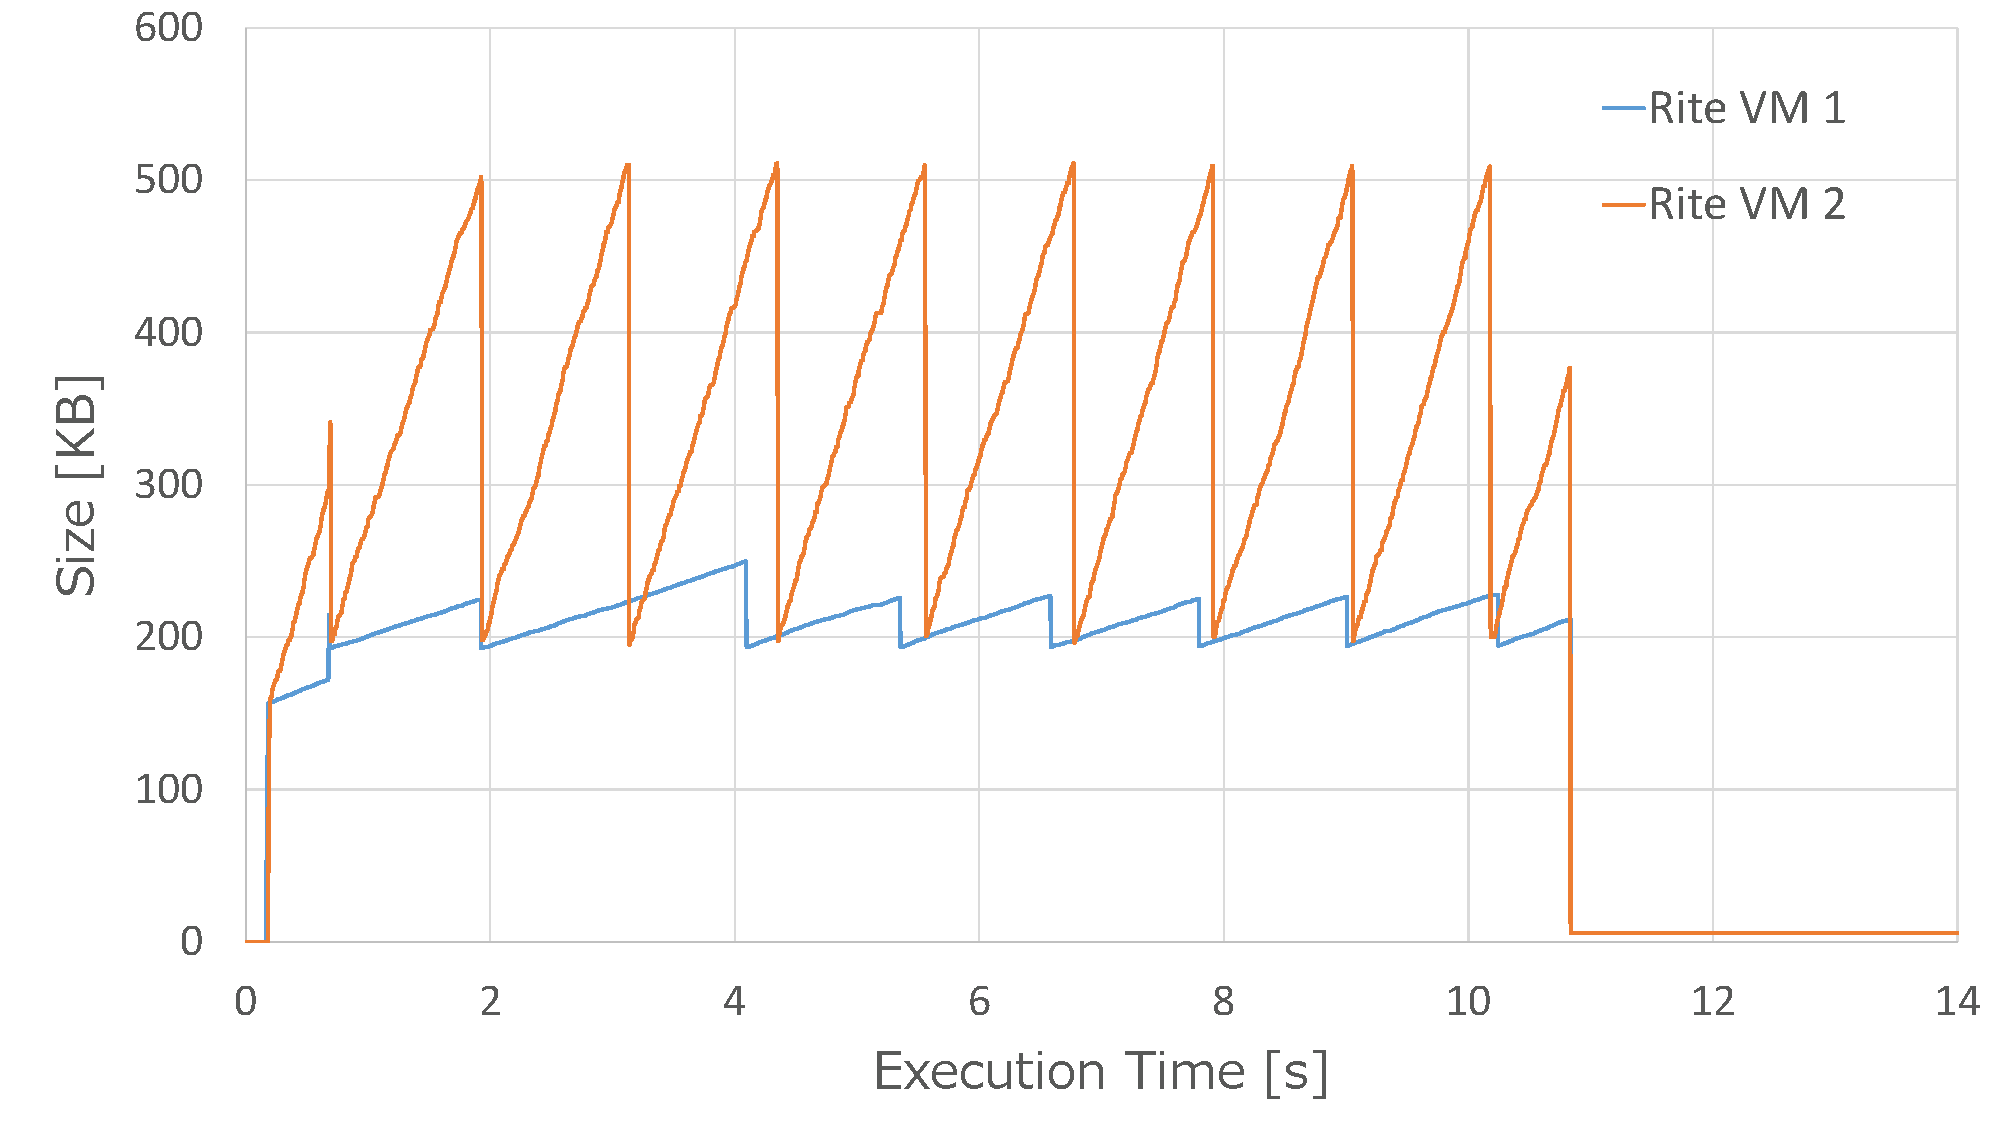
\includegraphics[width=8cm,clip]{figure/EvaluationOfTLSFStatistics.pdf}
    \caption{Memory usage of RiteVMs with TLSF+TECS}
    \label{fig:EvaluationOfTLSFStatistics}
\end{figure}

\begin{figure}[t]
    \centering
    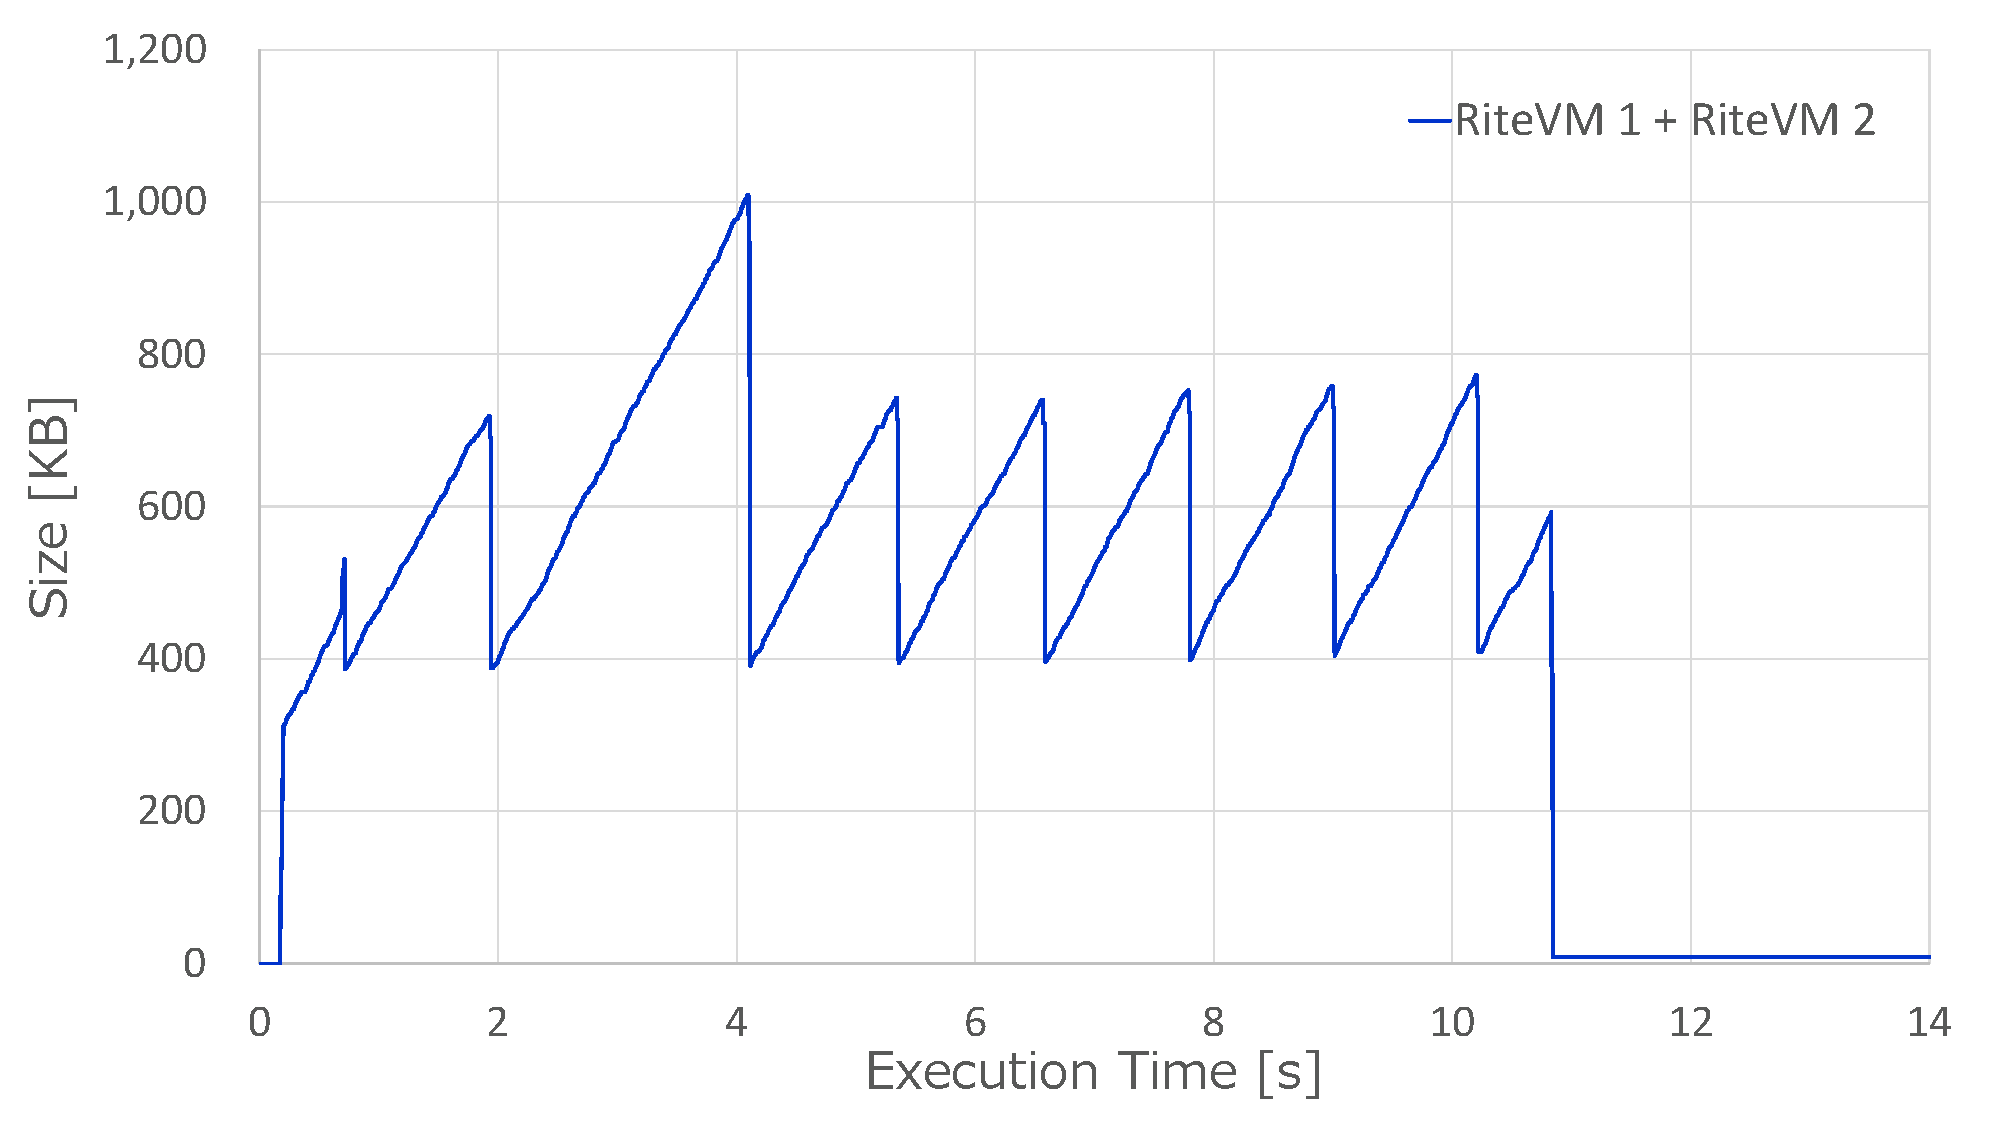
\includegraphics[width=8cm,clip]{figure/EvaluationOfMemoryUsageWithExclusiveContorol.pdf}
    \caption{Memory usage of RiteVMs with exclusive control}
    \label{fig:EvaluationOfMemoryUsageWithExclusiveContorol}
\end{figure}

\subsection{Memory usage of RiteVMs by TLSF+TECS}

The proposed dynamic memory allocator, TLSF+TECS, executes multiple tasks without exclusive control concurrently because each TLSF component holds its own heap area.
The TLSF+TECS framework provides functionality to acquire statistical information describing dynamic memory usage.
Therefore, it is possible to analyze the operational status of the TLSF and GC on RiteVMs.

Fig.\ref{fig:EvaluationOfTLSFStatistics} shows the memory usage of two RiteVMs, with presented data acquired from the statistical information available via the TLSF+TECS framework.
From the figure, we observe that when the RiteVM are first activated, a large amount of memory is allocated for each RiteVM and initialization is performed within one second.
Next, the applications runs for ~10 s and the RiteVMs subsequently terminate.
The reduction in memory usage that occurs at regular intervals is due to the GC function of the RiteVM.
Here, an application that allocates tens of KB of memory runs on RiteVM 1 and an application that allocates hundreds of KB of memory runs on RiteVM 2.
Fig.\ref{fig:EvaluationOfMemoryUsageWithExclusiveContorol} shows the memory usage when two RiteVMs are executed in one heap area with exclusive control.
In Fig.\ref{fig:EvaluationOfDynamicConnection}, two applications are finished at 10.837 s, and in Fig.\ref{fig:EvaluationOfMemoryUsageWithExclusiveContorol}, they are finished at 10.877 s, which demonstrates that the execution time of the applications has increased due to exclusive control.
In addition to the overhead of execution time, a RiteVM is not affected by other RiteVMs since TLSF+TECS keeps heap area independently.
GC on a RiteVM is performed periodically; however, there is a part that GC is not performed periodically in RiteVM 1 of Fig.\ref{fig:EvaluationOfExecutionTime}.
In Fig.\ref{fig:EvaluationOfMemoryUsageWithExclusiveContorol}, two RiteVMs share one heap area; therefore, RiteVM 2 is affected by RiteVM 1.
On the other hand, in Fig.\ref{fig:EvaluationOfTLSFStatistics}, RiteVM 2 is not affected by RiteVM 1.

As such, the TLSF+TECS framework provides users with the ability to visualize GC behavior and help verify its operation.
Further, when the RiteVM terminates, the memory used by the RiteVM is not completely released, i.e., a few kilobytes remain.
This remaining memory causes a memory leak when the number of RiteVMs increases or a RiteVM repeatedly activates and shuts down.
Using the proposed environment here proves useful for detecting bugs related to memory, which in practice can be extremely difficult to detect.



%5
\section{Related Work}
\label{sec:Related Work}

To develop the software of IoT systems, several approaches have been proposed \cite{par:frameworkCPS} such as Wireless Sensor Network (WSN) macroprogramming, Cloud-based platforms, and Model-Driven Development (MDD), General-purpose Programming Languages (GPLs).

WSN macroprogramming provides abstractions to specify high-level collaborative behaviors, while hiding low-level details such as message passing and state maintenance.
nesC, a programming language used to build applications for the TinyOS platform \cite{par:nesc}, has been proposed.
nesC/TinyOS is designed for WSN nodes with limited resources e.g., 8 KB of program memory, 512 bytes of RAM, but not supported TCP/IP implementation.

A cloud-based platform reduces development efforts by providing cloud-base APIs and high-level constructs (e.g., drag-and-drop) \cite{par:cloud-based}.
In addition, it offers easy deployment and evolution because the application logic is centrally located in a cloud platform.
However, it is a platform-dependent design, and restricts developers in terms of functionality such as in-network aggregation or direct node-to-node communication locally.
The cloud-based mruby framework, enzi Board \cite{url:enzi}, has been proposed.
enzi can be developed and simulated on the Web, and the developer can download and run the program on the board.

To address the issues of development efforts and platform-dependent design, MDD has been proposed \cite{par:MDD}.
MDD provides the benefits of reusable, platform-independent, extensible design, however it needs a long development time to build MDD systems.

The development using GPLs such as C, JavaScript, Python, and Android allows the extremely efficient systems based on the complete control over individual devices.
However, GPLs need more development effort, and it is difficult to reuse software due to platform-dependent design.
Several Open-source runtime systems for scripting languages have been proposed such as python-on-a-chip \cite{url:python-on-a-chip}, the Owl system \cite{par:owl}, eLua \cite{url:eLua}.
mruby programs on TECS can be executed approximately 100 times faster than standard mruby programs \cite{par:mrubyonTECS}.
That is, mruby programs can be executed at the same speed as C, which is faster than other scripting languages.

The proposed framework can configure the TCP/IP protocol stack with minimum set compared to the other platforms.
Therefore, the proposed framework can reduce memory consumption.
In addition, the extended mruby on TECS supports a legacy code such as a motor driver.
mruby has the same syntax as Ruby which has advantages for web application development as it uses in Rails framework \cite{url:rubyonrails}.



%6
\section{Conclusion}
\label{sec:Conclusion}

This paper presented an extended framework of mruby on TECS, including TINET+TECS and TLSF+TECS.
In the proposed framework, mruby programs can call TINET+TECS functions through the mruby-TECS bridge.
The development of software for IoT devices such as sensors and actuators will be more efficient due to the high productivity of mruby.

TINET+TECS is a componentized version of TINET, a compact TCP/IP protocol stack that uses TECS.
It improves on TINET configurability while suppressing the overhead of componentization.
Scalability is also improved because the component-based framework simplifies to add/remove and change protocols such as TCP/UDP, IPv4/IPv6, and Ethernet/PPP.
This paper also presented the dynamic connection, a new TECS functionality, to enable dynamic processing while reducing memory consumption.
TINET+TECS utilizes the dynamic connection to satisfy the TINET specification for supporting the static generation of CEPs and REPs.
TLSF+TECS is a component-based dynamic allocator.
Since the TLSF+TECS can hold its own heap area, memory contention will not occur even if memory is simultaneously allocated or released from multiple threads.
TINET+TECS and TLSF+TECS can be applicable to various embedded systems because these frameworks are executed on TECS and not limited to mruby.

In addition, the RiteVMs, TINET+TECS, and TLSF+TECS are implemented as components; therefore, developers can add, remove, or reuse their functionalities easily as required.
Note that our prototype system and the application programs used in the performance evaluation are all open-source and can be downloaded from our website \cite{url:TECS}.
In the future, we will support mruby libraries as mrbgems, which is an mruby distribution packaging system.\newline

\begin{acknowledgment}
This work was supported by JSPS KAKENHI Grant Number 15H05305.
We would like to thank Hiroaki Nagashima and Kazuaki Tanaka for supporting this research.
\end{acknowledgment}


%Reference
\bibliographystyle{ipsj_v2/UTF8/ipsjunsrt-e}
\bibliography{ref}

\begin{biography}
\profile{Takuro Yamamoto}
{
received his B.E. degree from Osaka University in 2016.
His research interests include real-time and embedded systems\@.
}
\profile{Takuma Hara}
{
\@.
}
\profile{Takuya Ishikawa}
{
\@.
}
\profile{Hiroshi Oyama}
{
received Dr. Engineering degree from Gifu University in 2002.
He works at Okuma Corporation as Senior Engineer and also works at Nagoya University as Visiting Professor.
He is studying software components and programming language for embedded systems\@.
}
\profile{Hiroaki Takada}
{
is a professor at Institute of Innovation for Future Society, Nagoya University.
He is also a professor and the Executive Director of the Center for Embedded Computing Systems (NCES), the Graduate School of Informatics, Nagoya University.
He received his Ph.D. degree in Information Science from University of Tokyo in 1996.
He was a Research Associate at University of Tokyo from 1989 to 1997, and was a Lecturer and then an Associate Professor at Toyohashi University of Technology from 1998 to 2003.
His research interests include real-time operating systems, real-time scheduling theory, and embedded system design.
He is a member of ACM, IEEE, IEICE, JSSST, and JSAE\@.
}
\profile{Takuya Azumi}
{
is an Assistant Professor at the Graduate School of Engineering Science, Osaka University. 
He received his Ph.D. degree from the Graduate School of Information Science, Nagoya University.
From 2008 to 2010, he was under the research fellowship for young scientists for Japan Society for the Promotion of Science.
From 2010 to 2014, he was an Assistant Professor at the College of Information Science and Engineering, Ritsumeikan University.
His research interests include real-time operating systems and component based development.
He is a member of IEEE, ACM, IPSJ, and IEICE\@.
}


\end{biography}


% \begin{biography}
% \profile{Taro Joho}{was born in 1970. He received his M.S. degree from
% Johoshori University in 1994.
% He joined
% the Information
% Processing Society of Japan in 1994.
% He is currently an associate professor at
% \mbox{Johoshori} University.
% His research interest is online
% publishing systems. He is a member of the IEEE and ACM\@.}
% %
% \profile{Hanako Shori}{was born in 1960. She received her M.E.\ and
% Ph.D.\ from Johoshori University in 1984 and 1987, respectively. She
% became an associate professor at Gakkai University in 1992 and a
% professor at Johoshori University in 1997. Her current research
% interest is online publishing systems. She received the Kiyasu Kinen
% award in 2010. She is a Board Member of the IPSJ and a member of the
% IEICE, IEEE-CS, and ACM\@.}
% %
% \profile{Jiro Gakkai}{was born in 1970. He received his M.S.\ degree
% from Johoshori University in 1994 and has been engaged in the
% Information Processing Society of Japan since 1994. His research
% interest is online publishing systems. He is a member of the IEEE and
% ACM\@.}
% %
% \end{biography}

\end{document}
